\section{Methods}

\subsection{Essential components}

This section contains lists of all the components required by the final robot.

\textbf{Power and logic boards:}
\begin{multicols}{3}
    \begin{itemize}
        \item Fit PC
        \item Power board
        \item DC motor control board
        \item Servo control board
    \end{itemize}
\end{multicols}

\textbf{Sensors and camera:}
\begin{multicols}{3}
    \begin{itemize}
        \item Light sensors (x3)
        \item IR sensors (x2)
        \item Camera
        \item Sonar
        \item Hall effect sensor
    \end{itemize}
\end{multicols}

\textbf{Actuators and battery:}
\begin{multicols}{3}
    \begin{itemize}
        \item DC motors (x2)
        \item Battery
    \end{itemize}
\end{multicols}

Up until the first major milestone, the robot also had two whisker sensors, but they have since been removed. Their initial purpose and the reason why they were removed are documented on section \hyperref[sec:whiskers]{Sensing: Whiskers}

% - - - - - - - - - - - - - - - - - - - - - - - - - - -

\subsection{Physical architecture}

The entire structure of the robot is made out of LEGO parts. The robot has two large rubber LEGO wheels on the front, and one LEGO steel ball caster on the back. The robot is driven by the two large wheels on the front, and the caster wheel is just for support.\\
This design was preferred from the beginning because it allows the robot to rotate on itself, i.e., it can rotate any amount of degrees without actually moving relatively to the arena.

\clearpage

\begin{figure}[ht]
    \centering
    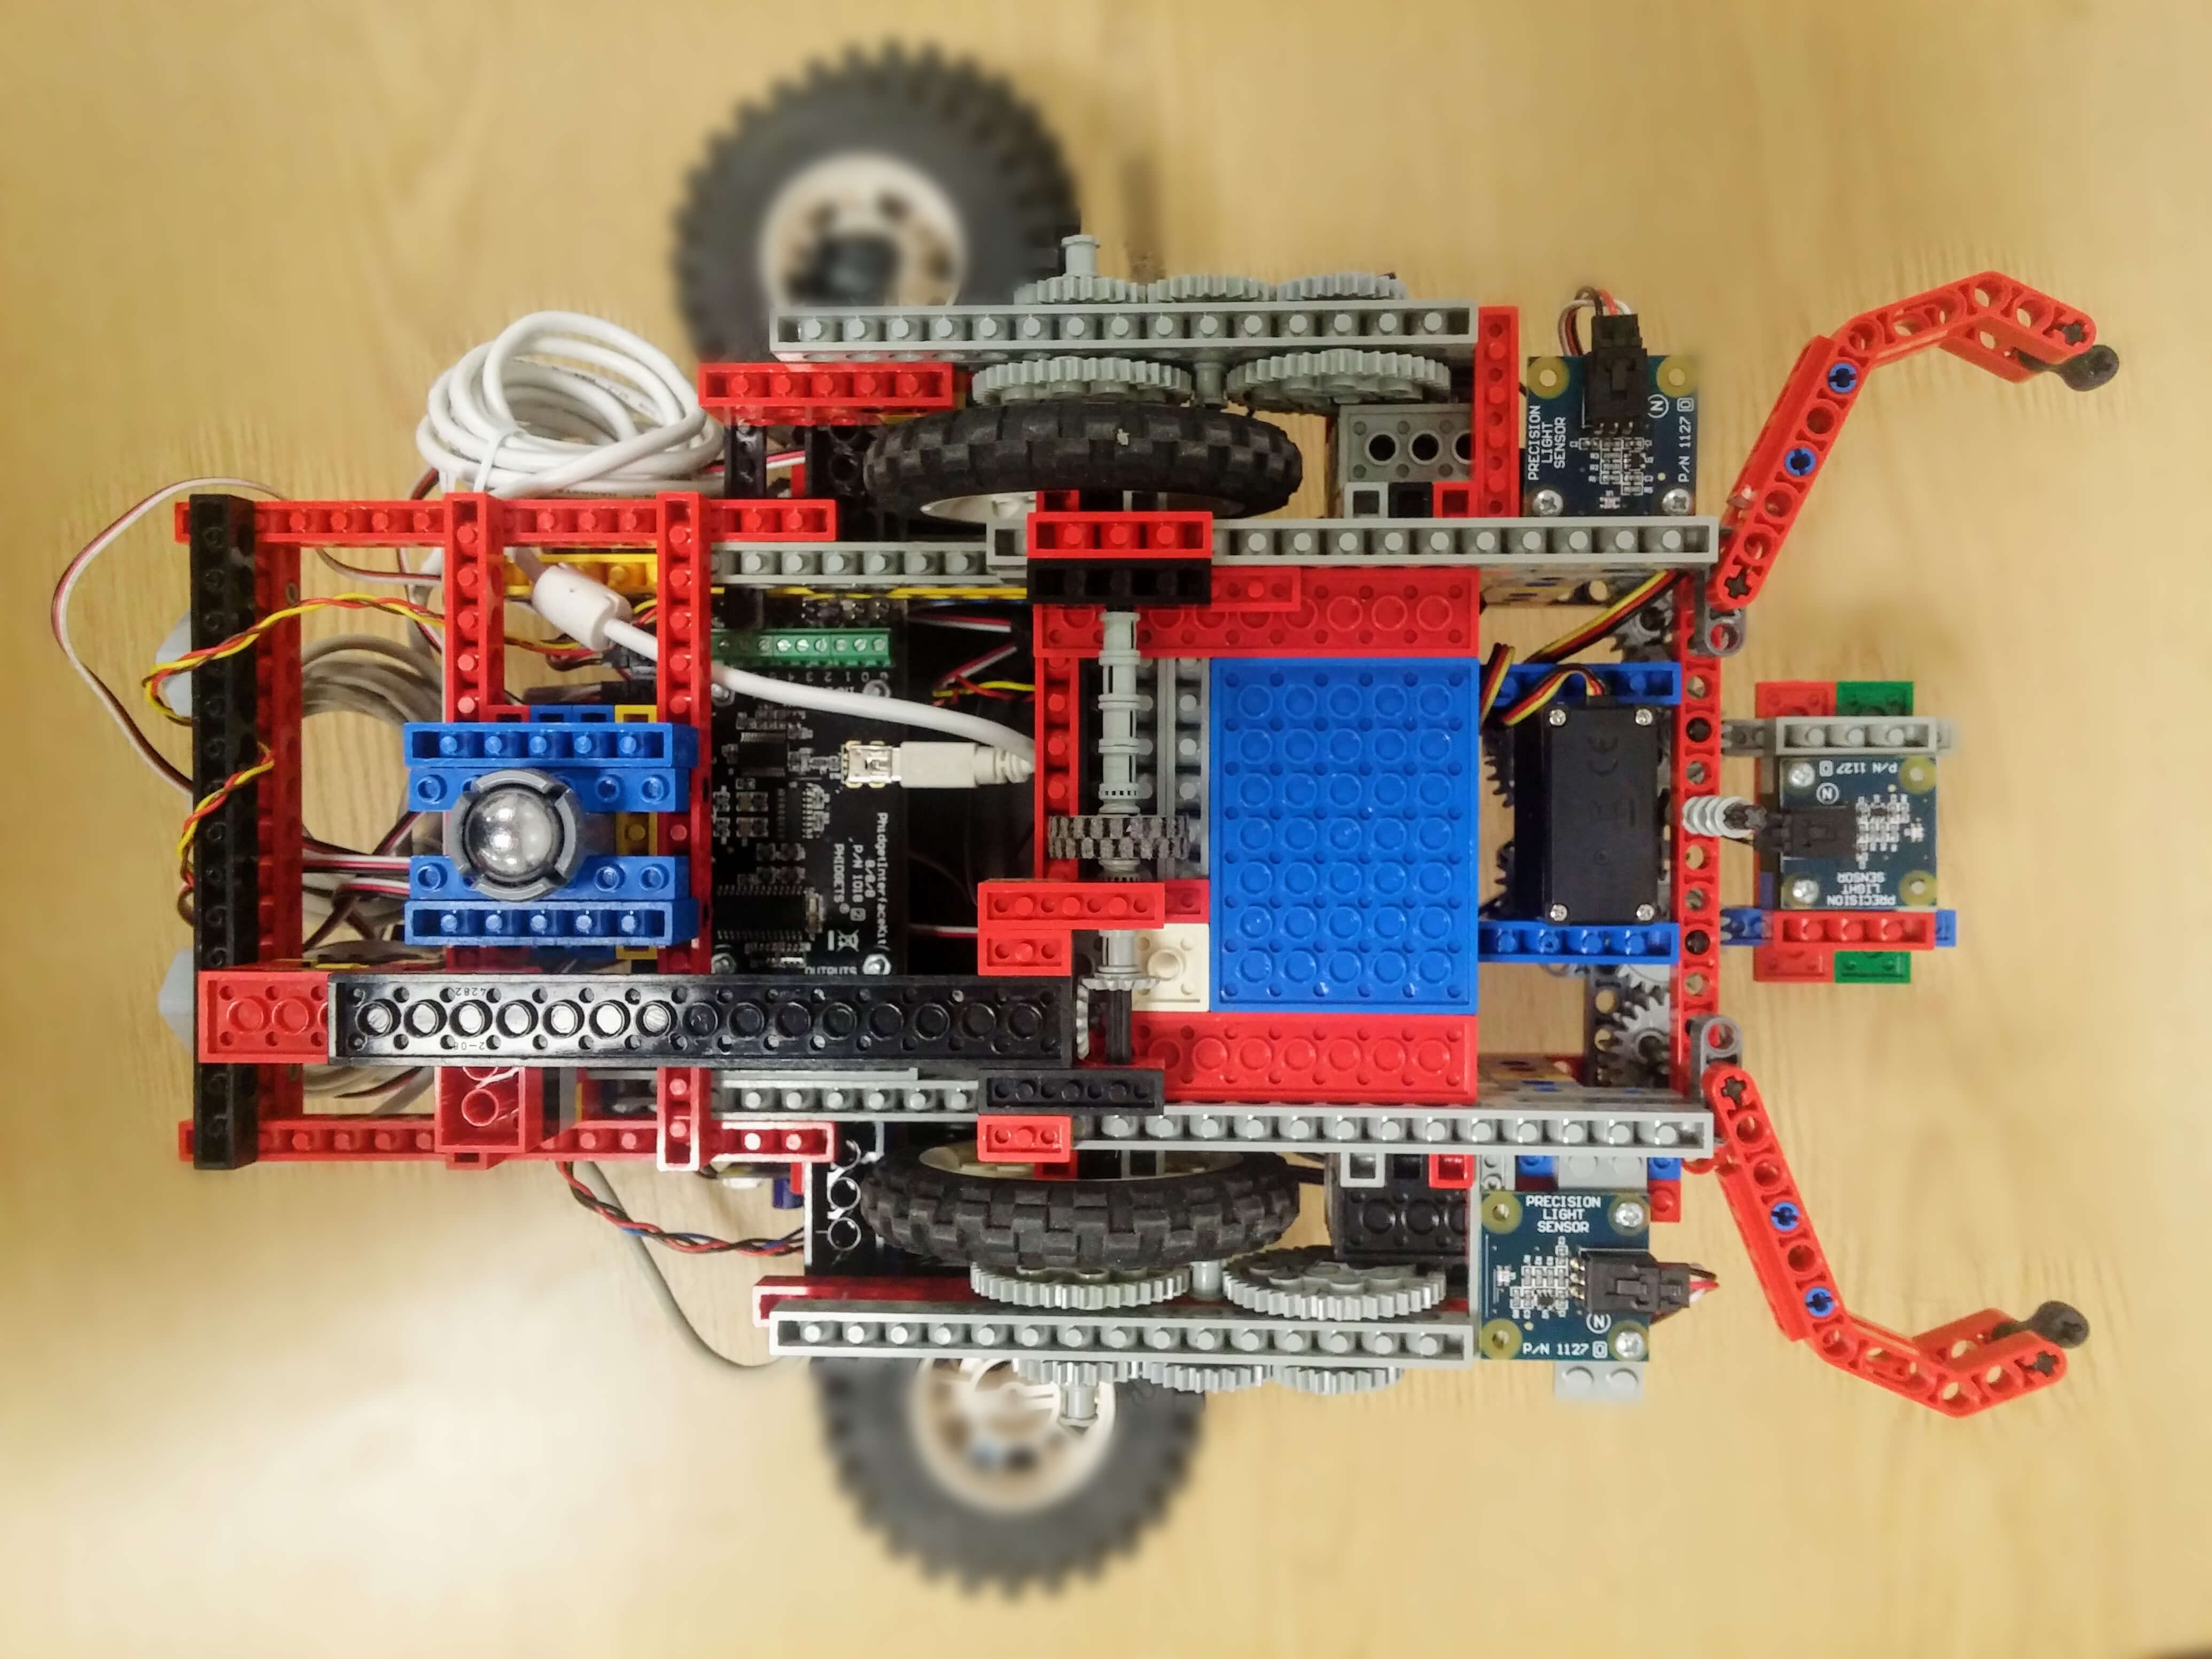
\includegraphics[height=0.7\linewidth, angle=90]{res/robot-pics/view-bottom.jpg}
    \caption{
        Bottom view of the robot. The caster wheel can be seen on the left of the image, and the two large rubber wheels on the center. The other wheels on the blurry background are not part of the robot and were used just to support the upside down robot while this shot was taken.
    }
\end{figure}

To take advantage of the quite heavy battery of the robot, it was placed as close to the front wheels as possible. Doing this added pressure on the tyres of the wheels, increasing the friction between them and the ground of the arena - which is considerably slippy from all the dust.

The power boards and the Fit PC were mounted on the back of the robot, between the two front wheels and the caster wheel. Doing this, and placing the battery close to the front wheels ensured that the center of mass would stay between all the wheels, approximately evenly distributed by them. This was a crucial element of the robot's design.

\bigskip

\begin{figure}[ht]
    \centering
    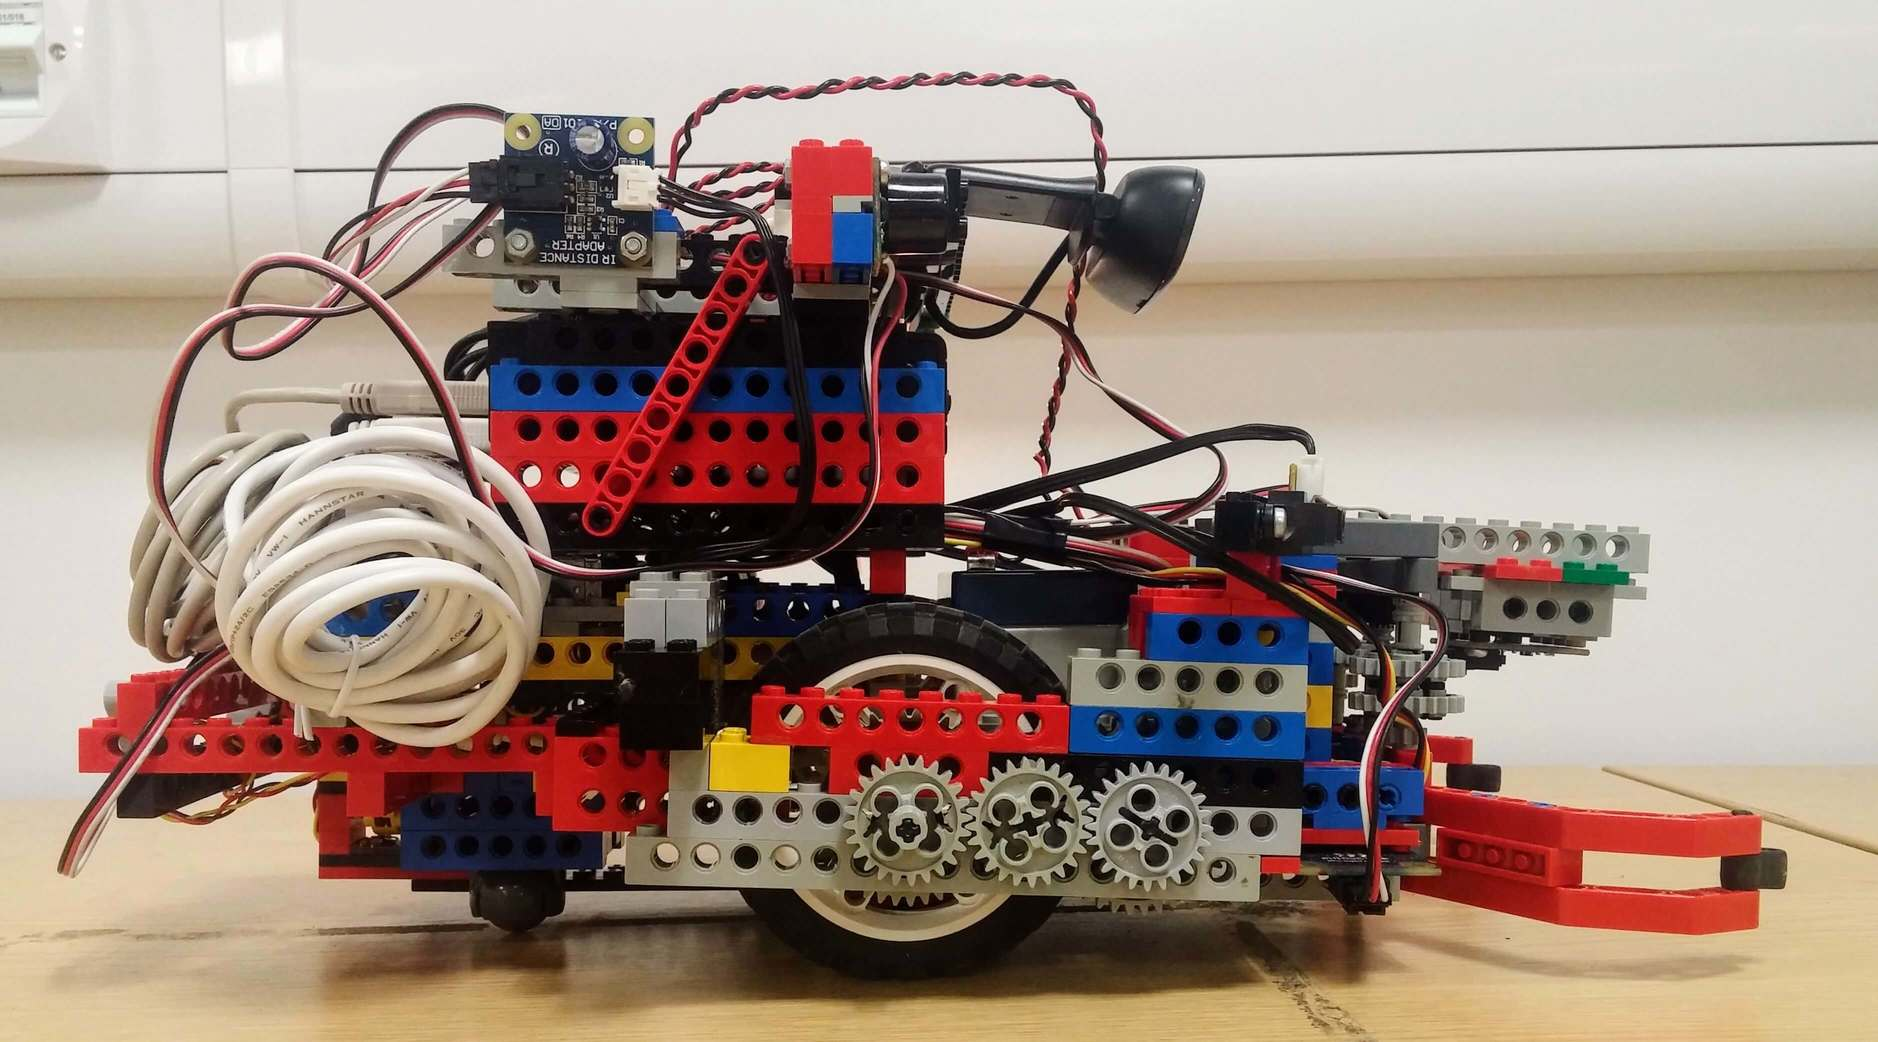
\includegraphics[width=0.7\linewidth]{res/robot-pics/view-right-side.jpg}
    \caption{View of the right side of the robot.}
\end{figure}

\clearpage

It was decided from the very start that the main Power Board should be easily accessible to plug the AC adaptor and to turn On/Off the DC motor power board. For that reason, the Power Board was placed on the very top of the robot, just behind the camera.

The need to constantly plug and unplug sensors to the Phidgets Boards made it clear that there should be an easy way to get to those sensor slots. This was even more important with the constant battery switching when they ran out of power. To solve this problem, a \textit{Hop On - Hop Off} with hinges was devised. To gain access to the boards and to the battery slot, one needed only to lift the hop.

\bigskip

\begin{figure}[ht]
    \centering
    \begin{subfigure}{0.49\textwidth}
        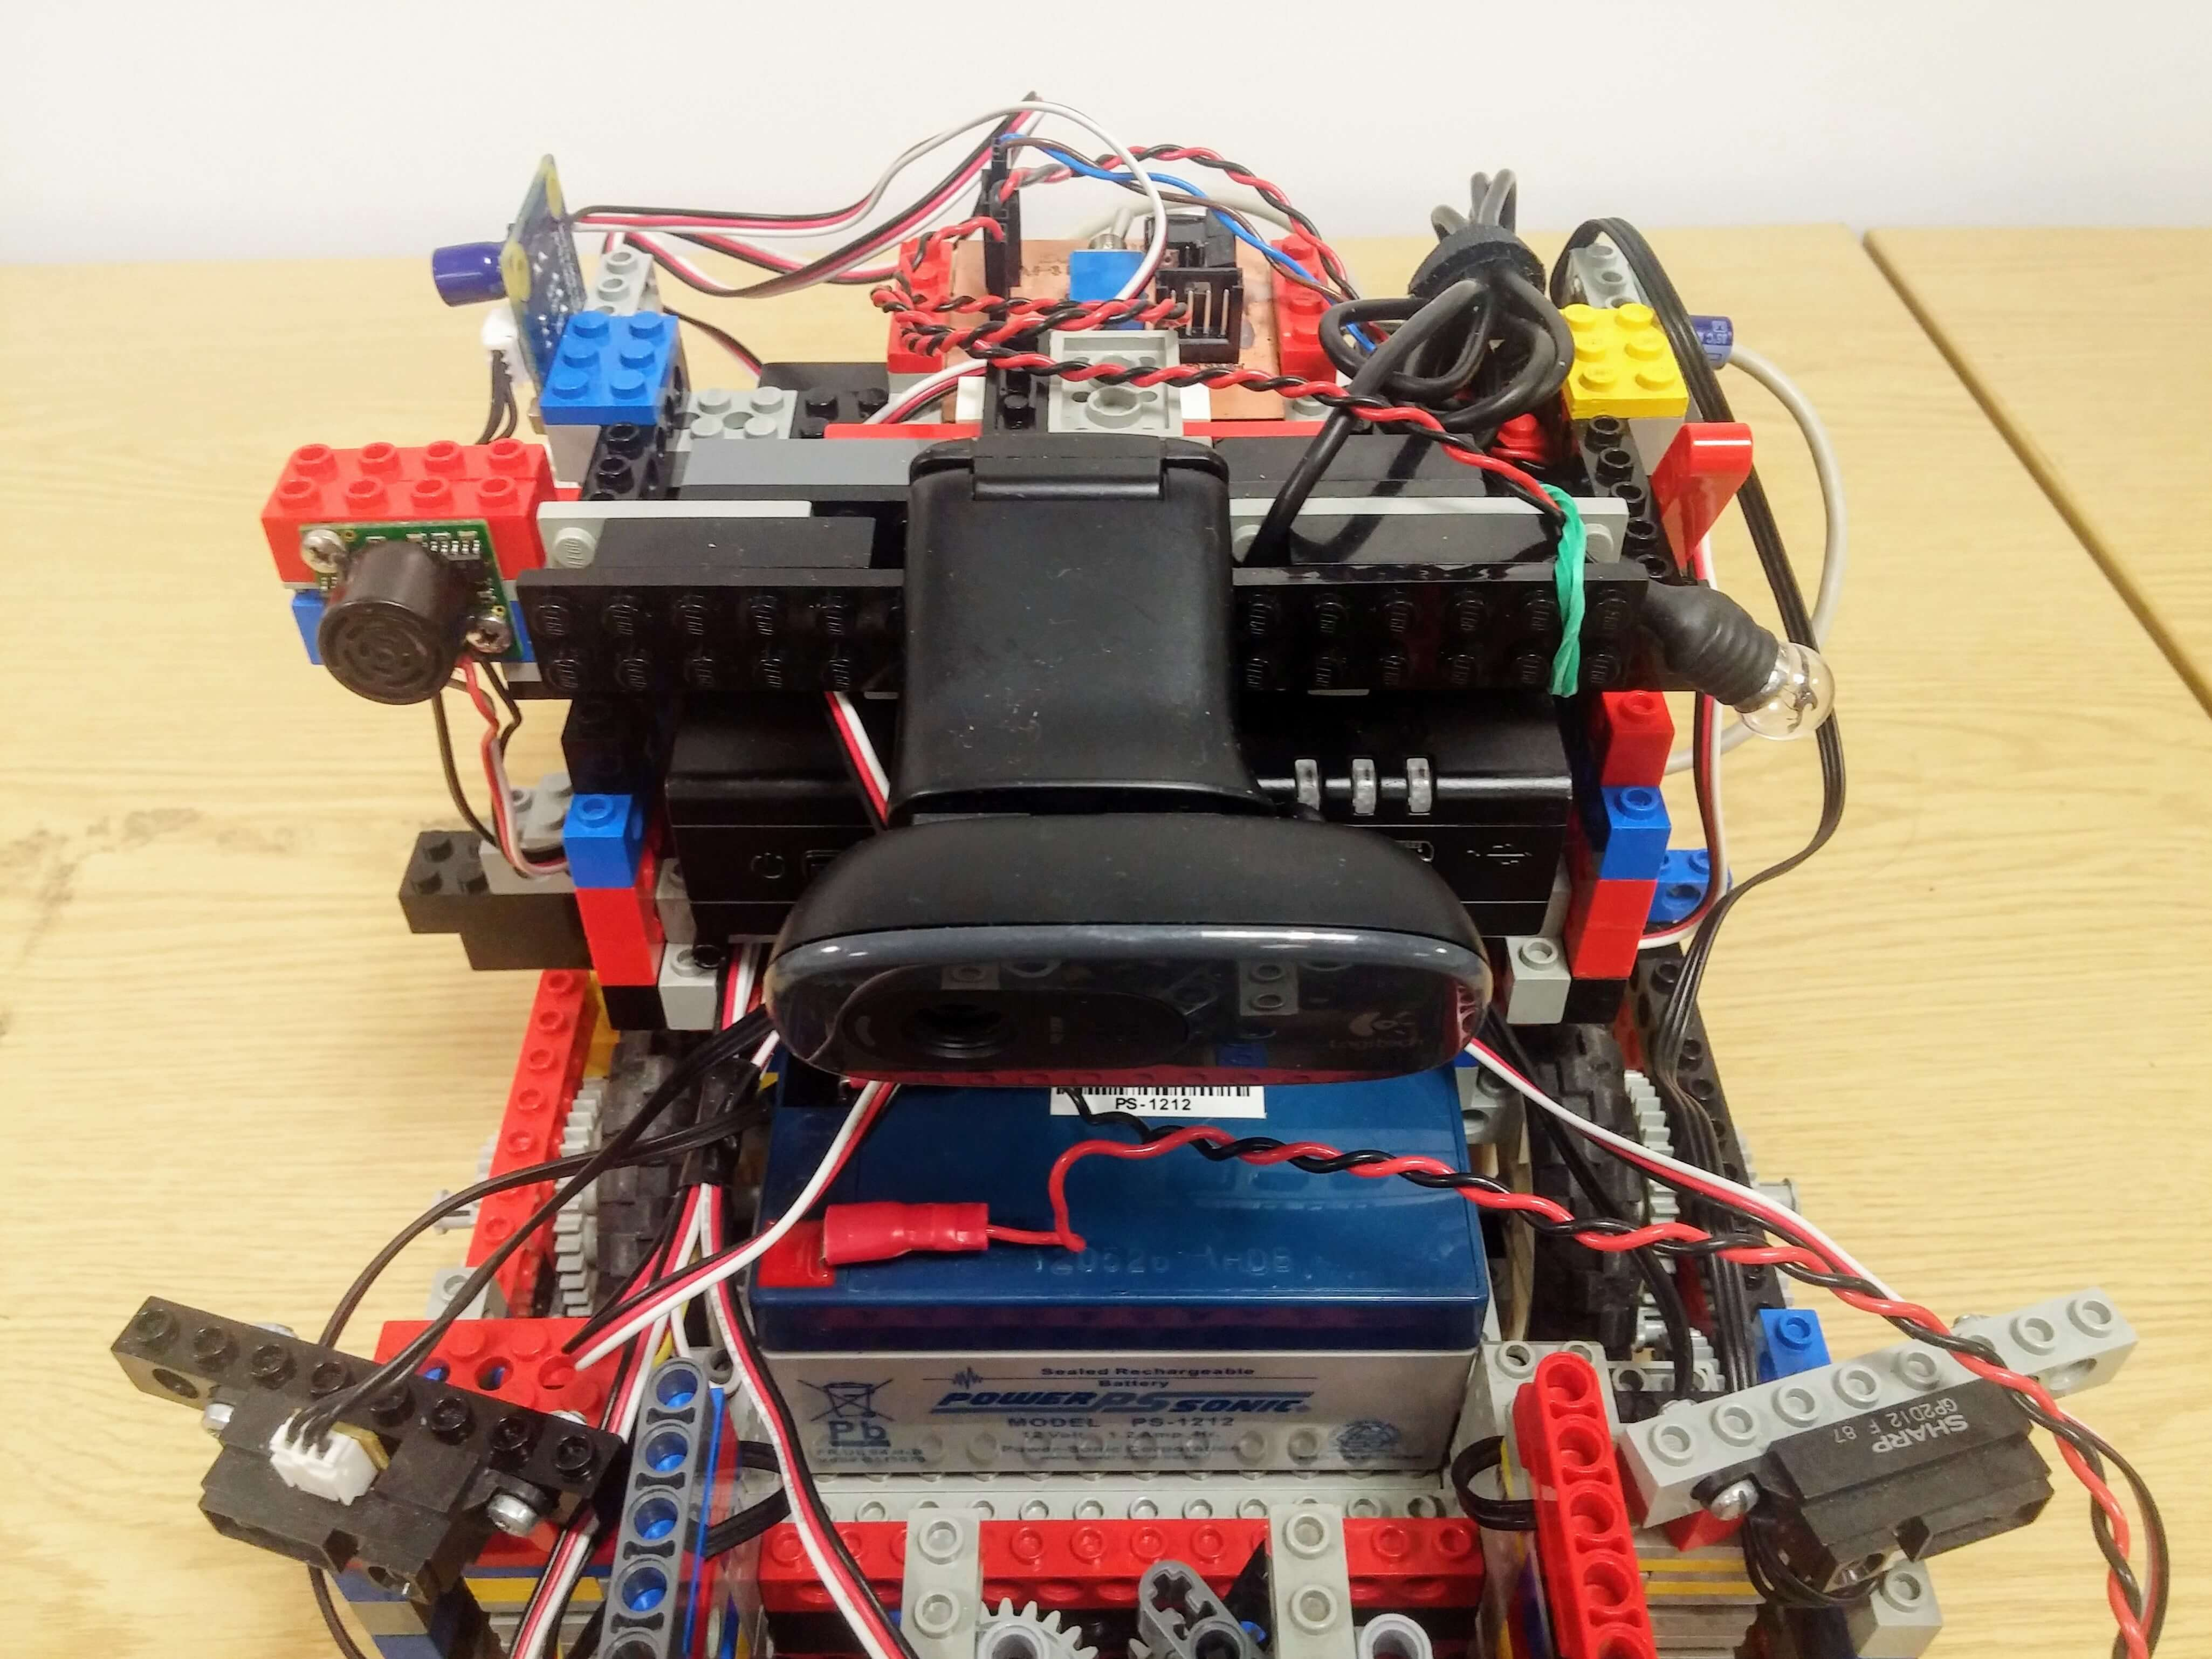
\includegraphics[width=\linewidth, height=4cm]{res/robot-pics/top-on.jpg}
        \caption{Hop on}
        \label{fig:hop-on}
    \end{subfigure}
    \begin{subfigure}{0.49\textwidth}
        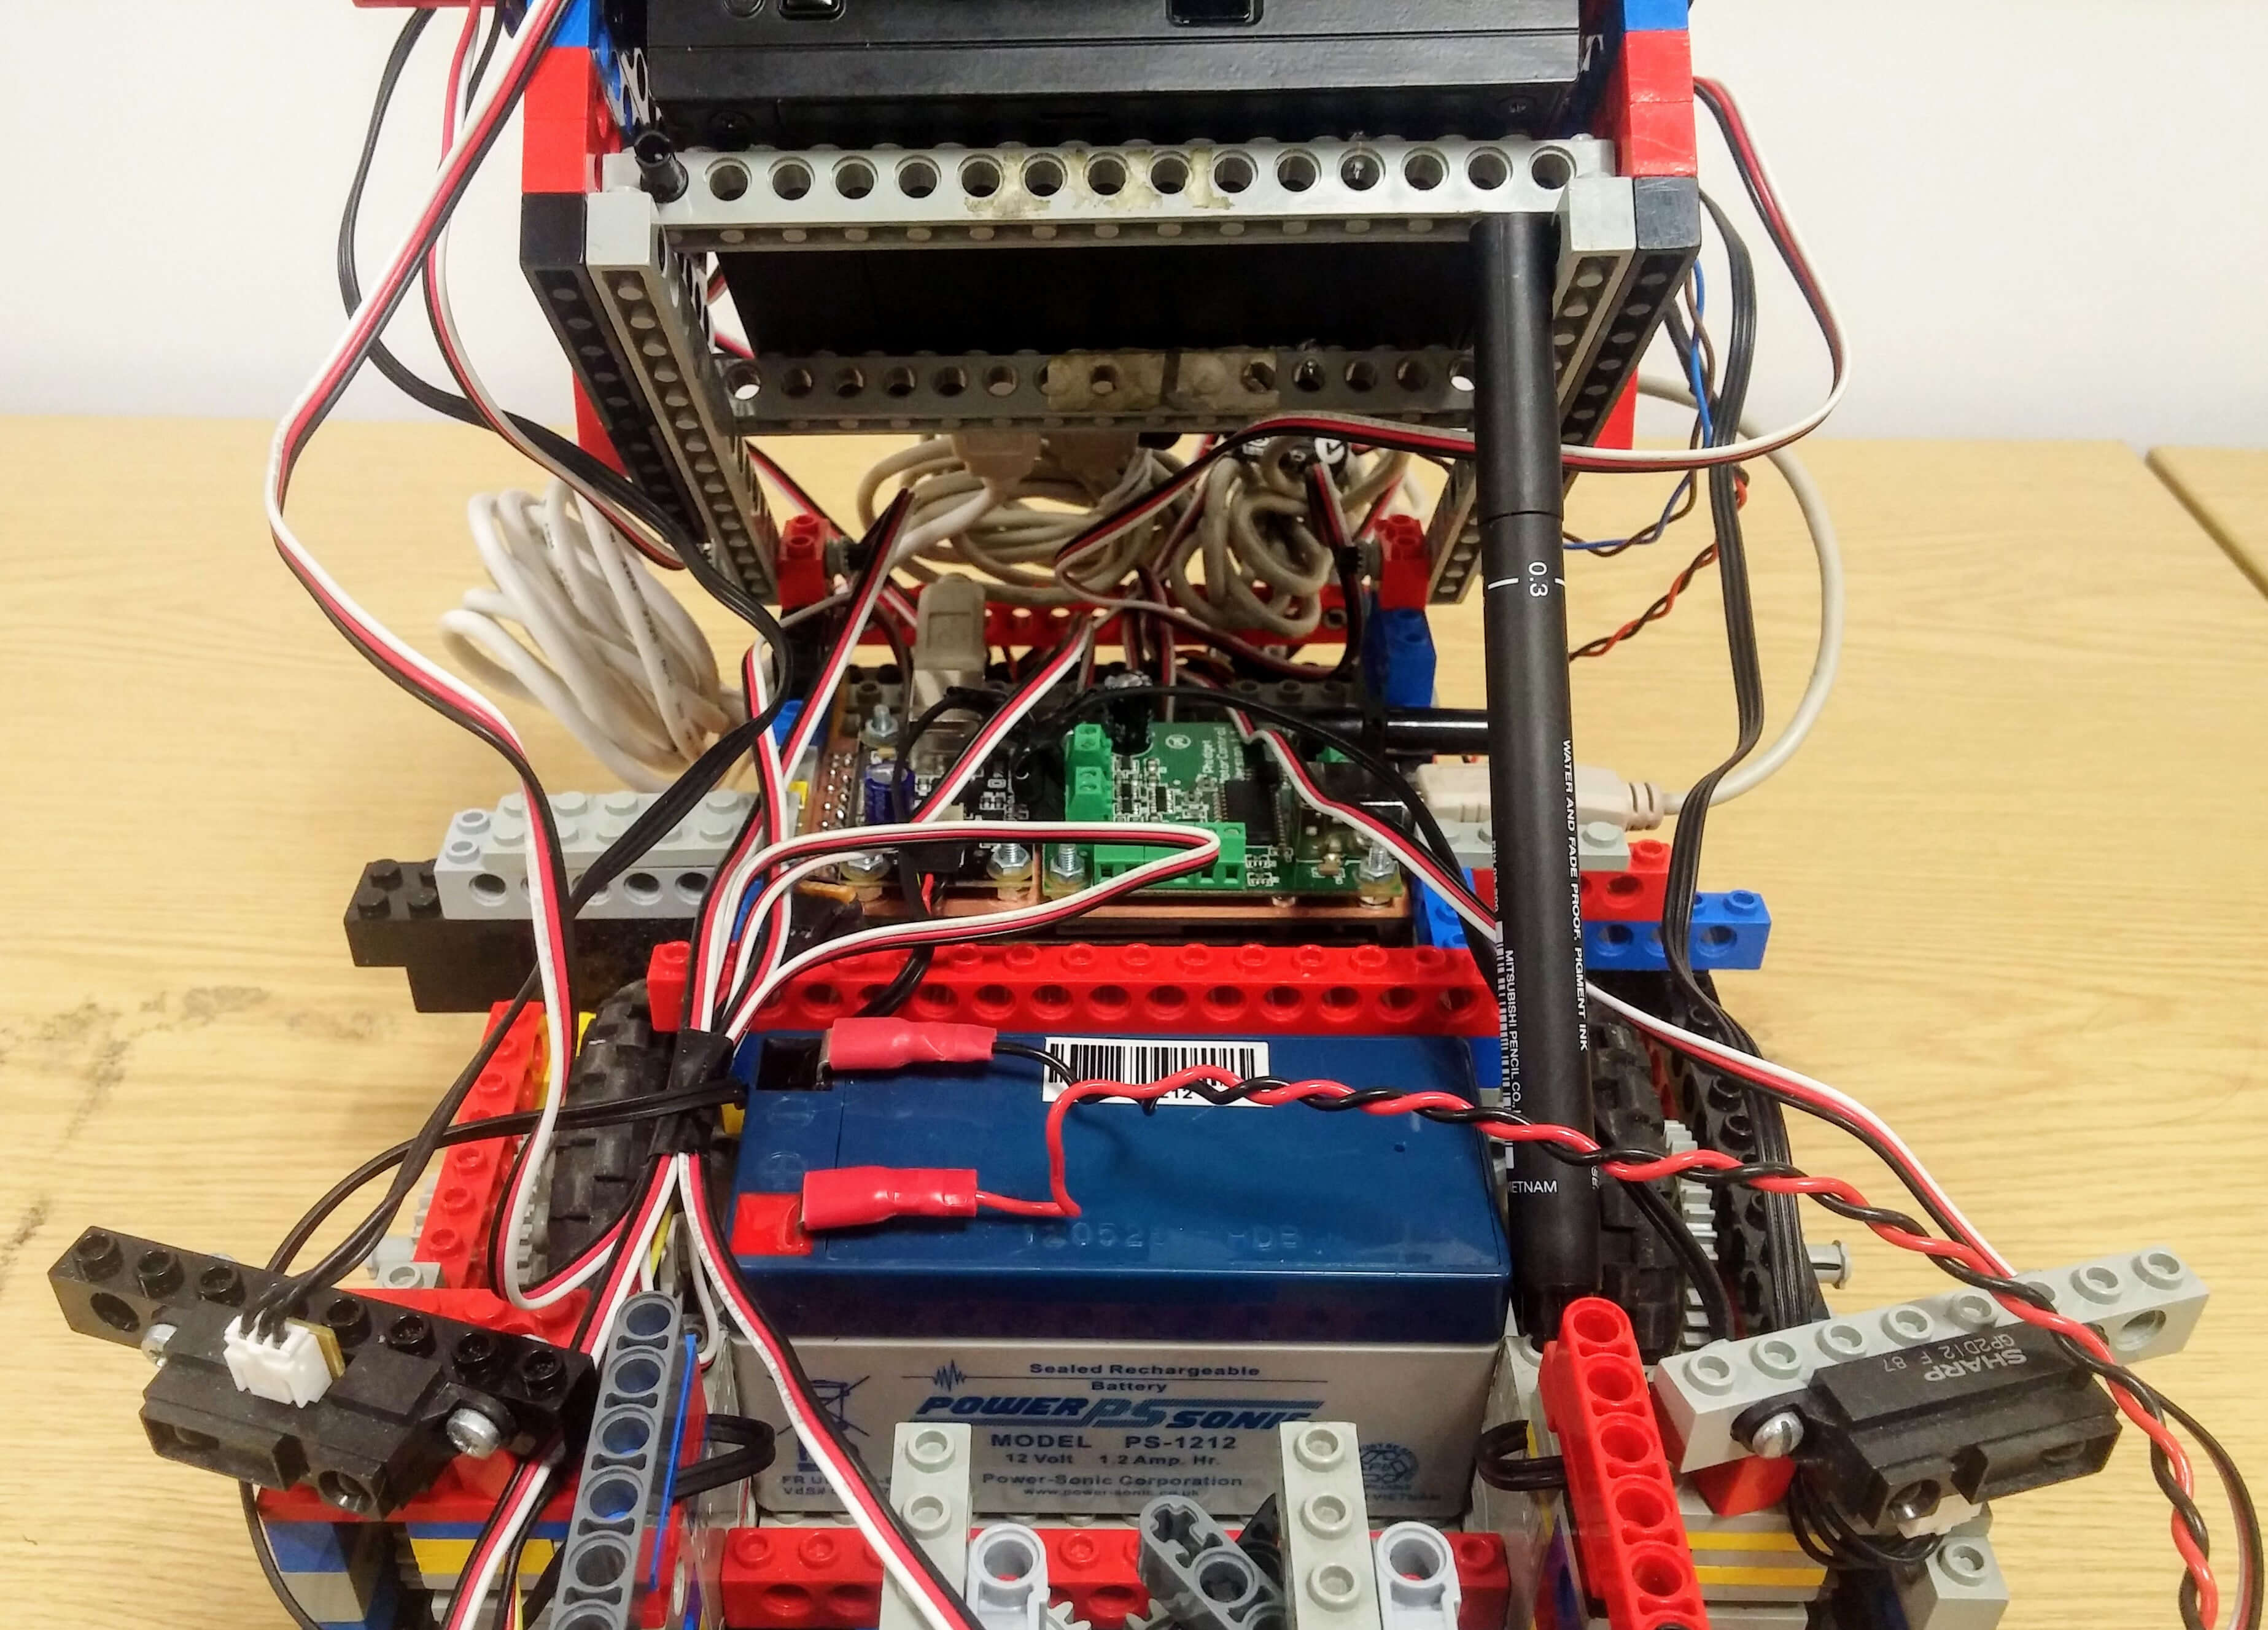
\includegraphics[width=\linewidth, height=4cm]{res/robot-pics/top-off.jpg}
        \caption{Hop off}
        \label{fig:hop-off}
    \end{subfigure}
    \caption{Lifting the hop reveals the Phidgets boards and enables easy access to the battery slot.}
    \label{fig:hop-on-off}
\end{figure}

% - - - - - - - - - - - - - - - - - - - - - - - - - - -

\subsection{Base detector and gripper}

The gripper had to be placed on the front in order to catch the cubes when the robot drove to them. The precision servo motor was used to open or close the gripper handles.

The tips of the gripper handles had a rubber LEGO part to prevent scenarios when the robot closed the gripper and the cube resource was not completely embraced by the handles. Having the rubber tips granted that the cube wouls still be secure in such situations.

One light sensor was mounted facing down on top of the gripper dock, at such a height that a cube would fit just underneath it. Since the cubes are textured on the sides, but are solid black on the top and bottom, placing the light sensor in such position made it very easy for the robot to detect whenever there was a cube on its gripper dock or not.

To complement the gripper, two more light sensors were placed at the front of the robot, one in each side, just hovering the floor and facing down.\\
These constituted the base detector for the black rectangular bases on the arena, and they functioned very similarly to the cube detector on the gripper: they measured the amount of light reflected by the gray floor of the arena, and triggered whenever black was being sensed instead of gray - this meant that that sensor was on one of the bases.\\
When the robot moved forward, carrying a cube and suddenly both light sensors from the base detector got triggered, it meant the robot had arrived to the base and it could release the cube to deliver it.

\bigskip

\begin{figure}[ht]
    \centering
    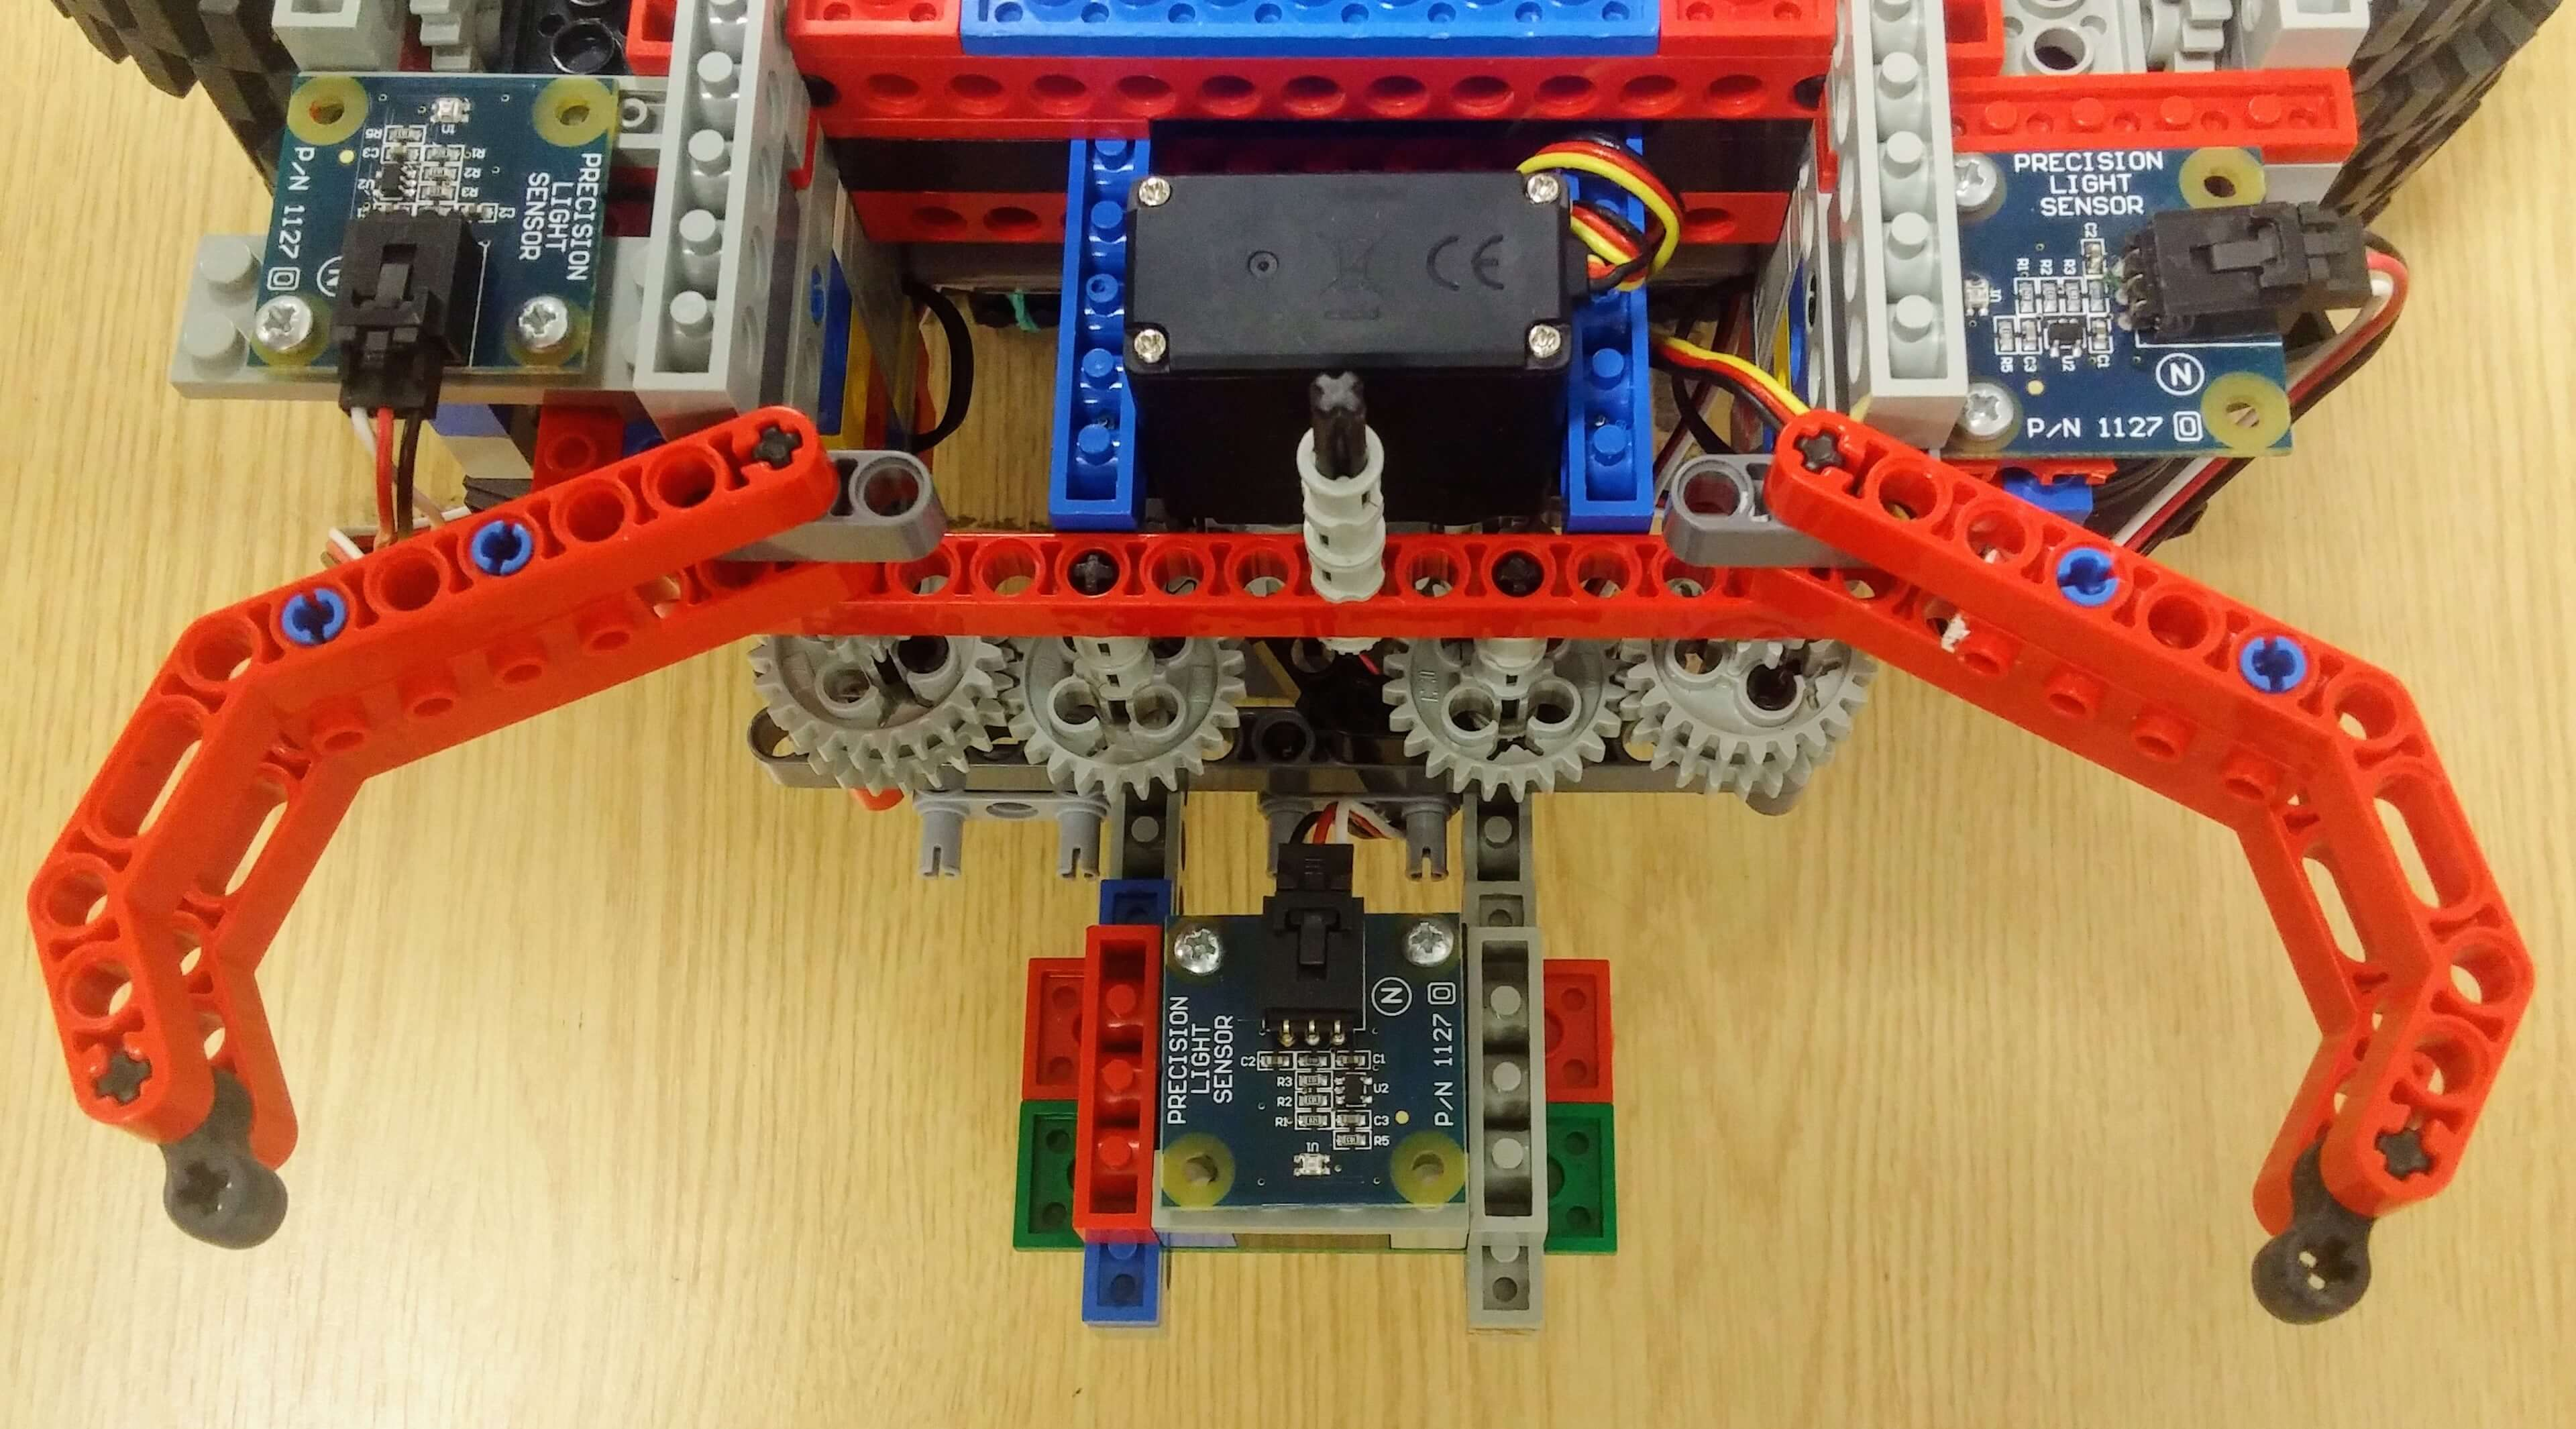
\includegraphics[width=0.7\linewidth]{res/robot-pics/base-detector-and-gripper.jpg}
    \caption{The base detector light sensors can be seen on the left and right top corners of this image. On the center, there is the precision servo motor, the gear train to open or close the gripper, and finally, on the middle bottom, the cube detection light sensor.}
    \label{fig:base-detector-and-gripper}
\end{figure}

% - - - - - - - - - - - - - - - - - - - - - - - - - - -

\subsection{Actuators and gearing}

The robot used two DC motors, each to drive its own wheel. However, the wheels were not directly connected to the motors. To have the best power/speed ratio, the power output of the motor had to be geared down with a gear train.\\
The DC motor output axle had a \textit{16-teeth} gear attached to it, which was connected to a \textit{40-teeth} gear. The rest of the gear train was just to transfer the power to a parallel axle, where the wheels were mounted to.

The total final gear ratio was \textbf{1:2.5}, which means the speed output by the DC motor was \textbf{decreased 2.5 times}, and the torque was \textbf{increased 2.5 times}. Furthermore, this gearing train made the wheels rotate 0.4 times per each revolution of the DC driver motor.

\bigskip

\begin{figure}[ht]
    \centering
    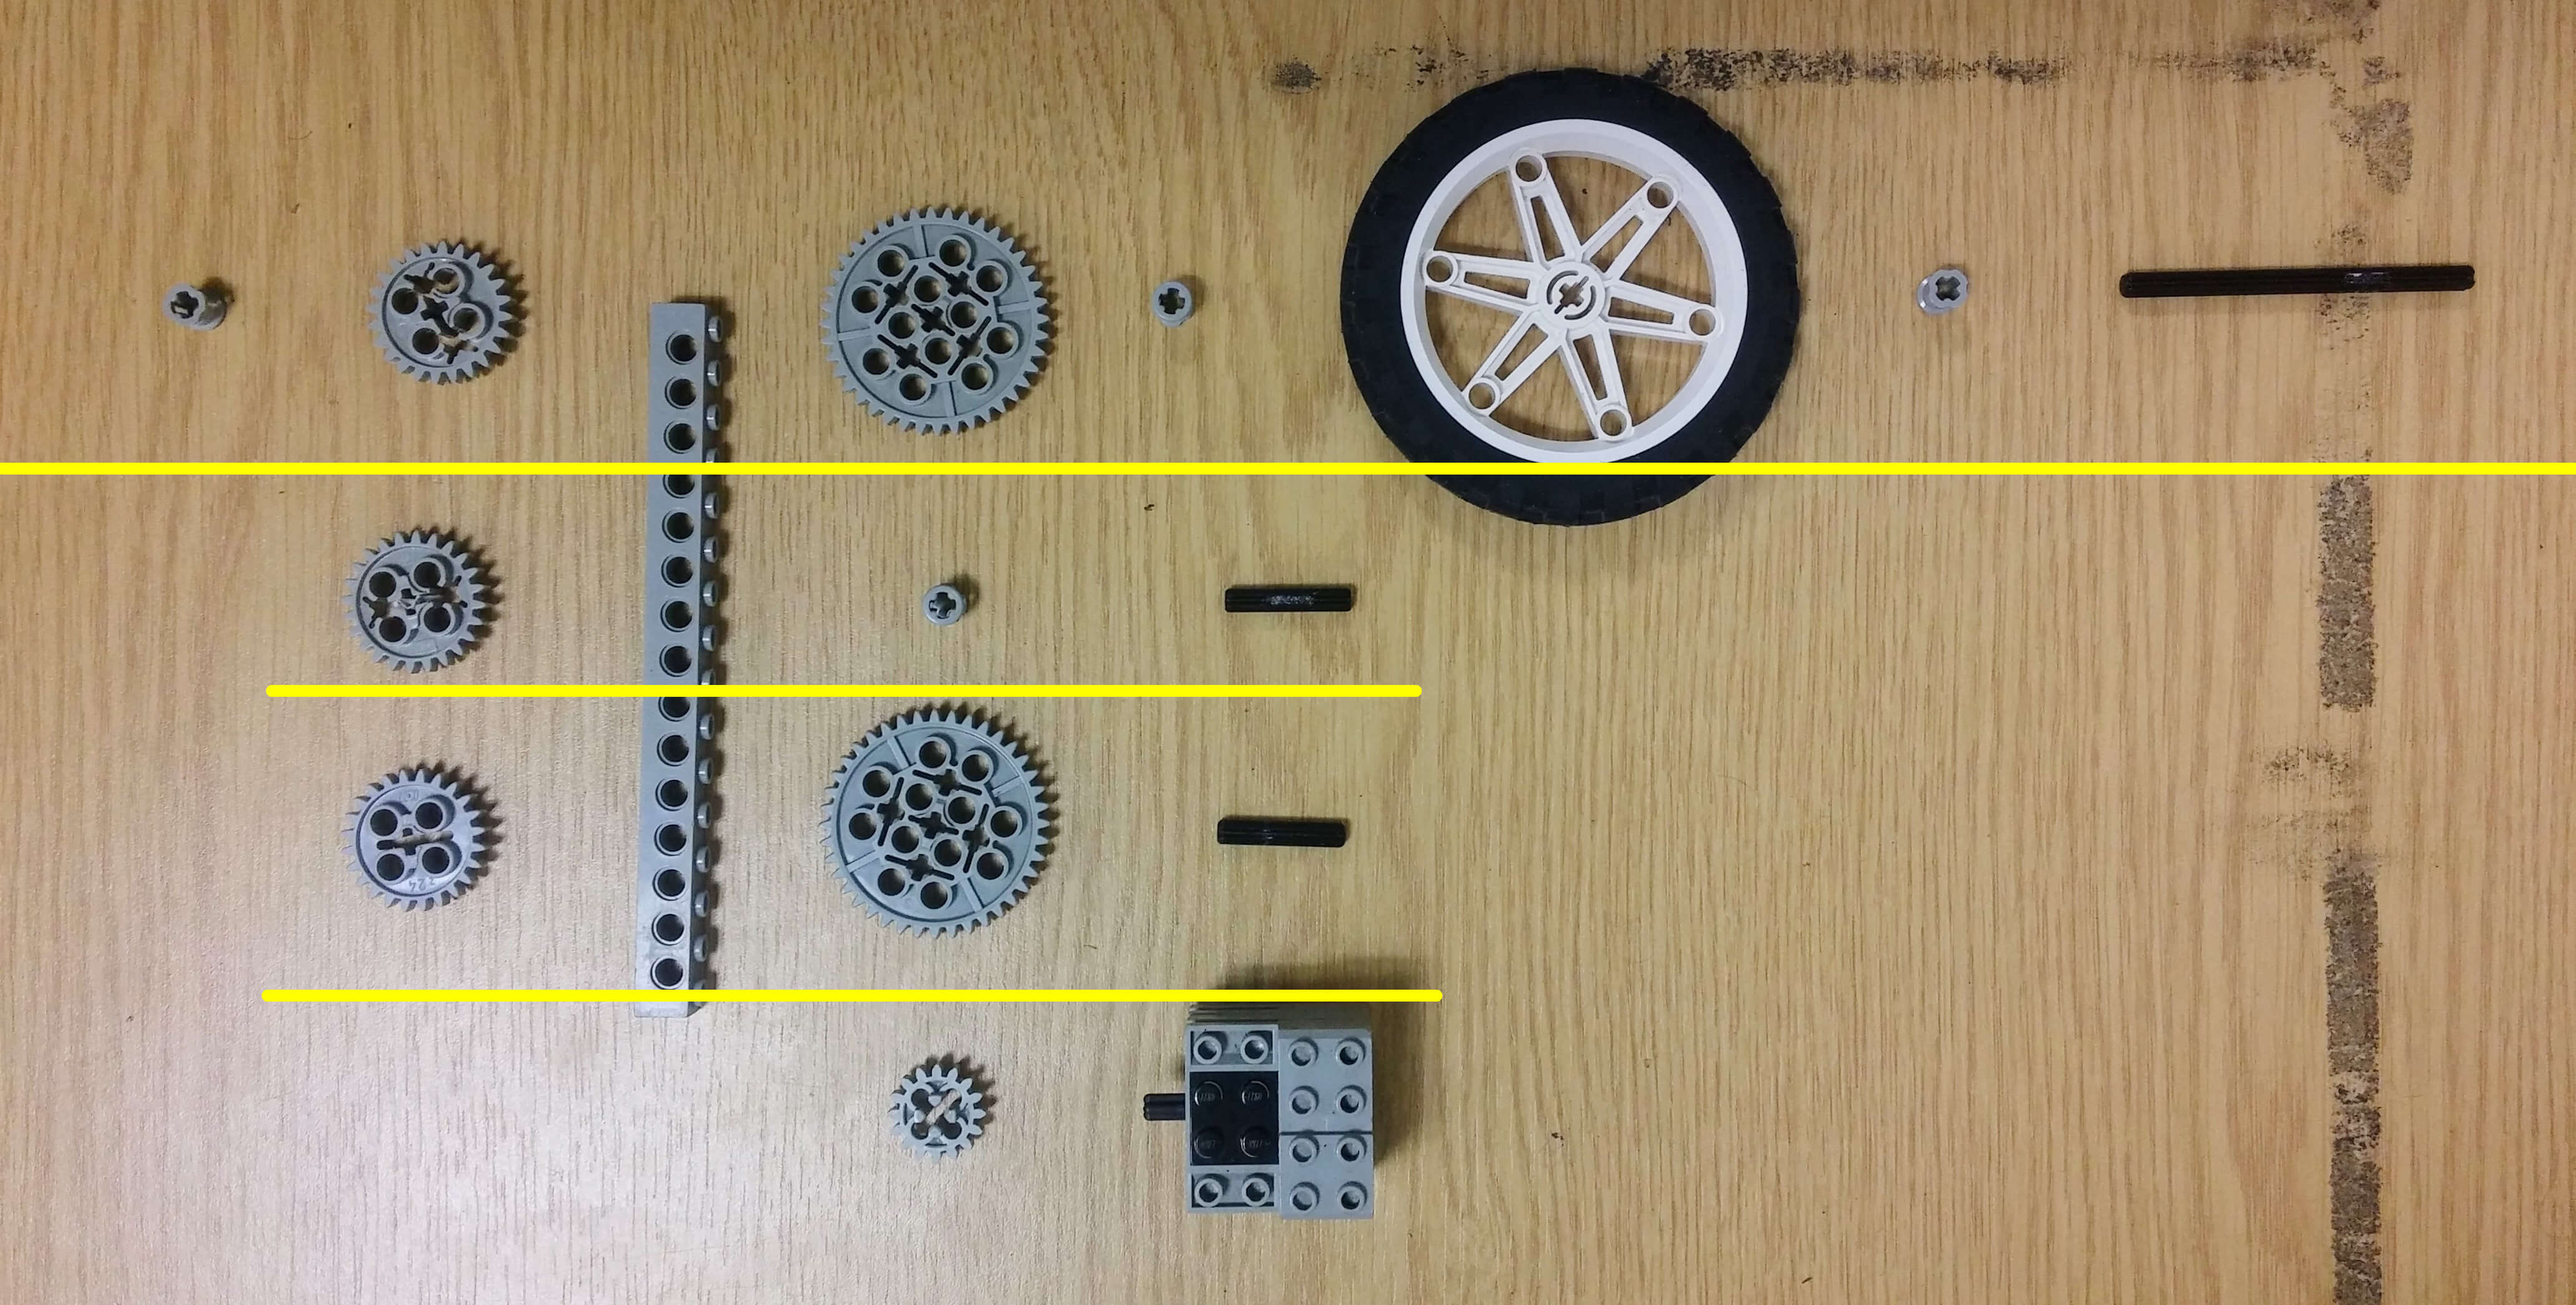
\includegraphics[width=0.7\linewidth]{res/robot-pics/gear-train-unmounted.jpg}
    \caption{All the components required to assemble the gear train of the robot, from the DC motor to the wheel. The yellow lines separate each stack of elements on an axle, e.g., all the LEGO parts above the first yellow line should be stacked to the black axle on the right, following the order by which they are layed out.}
    \label{fig:gear-train-unmounted}
\end{figure}

\begin{figure}[ht]
    \centering
    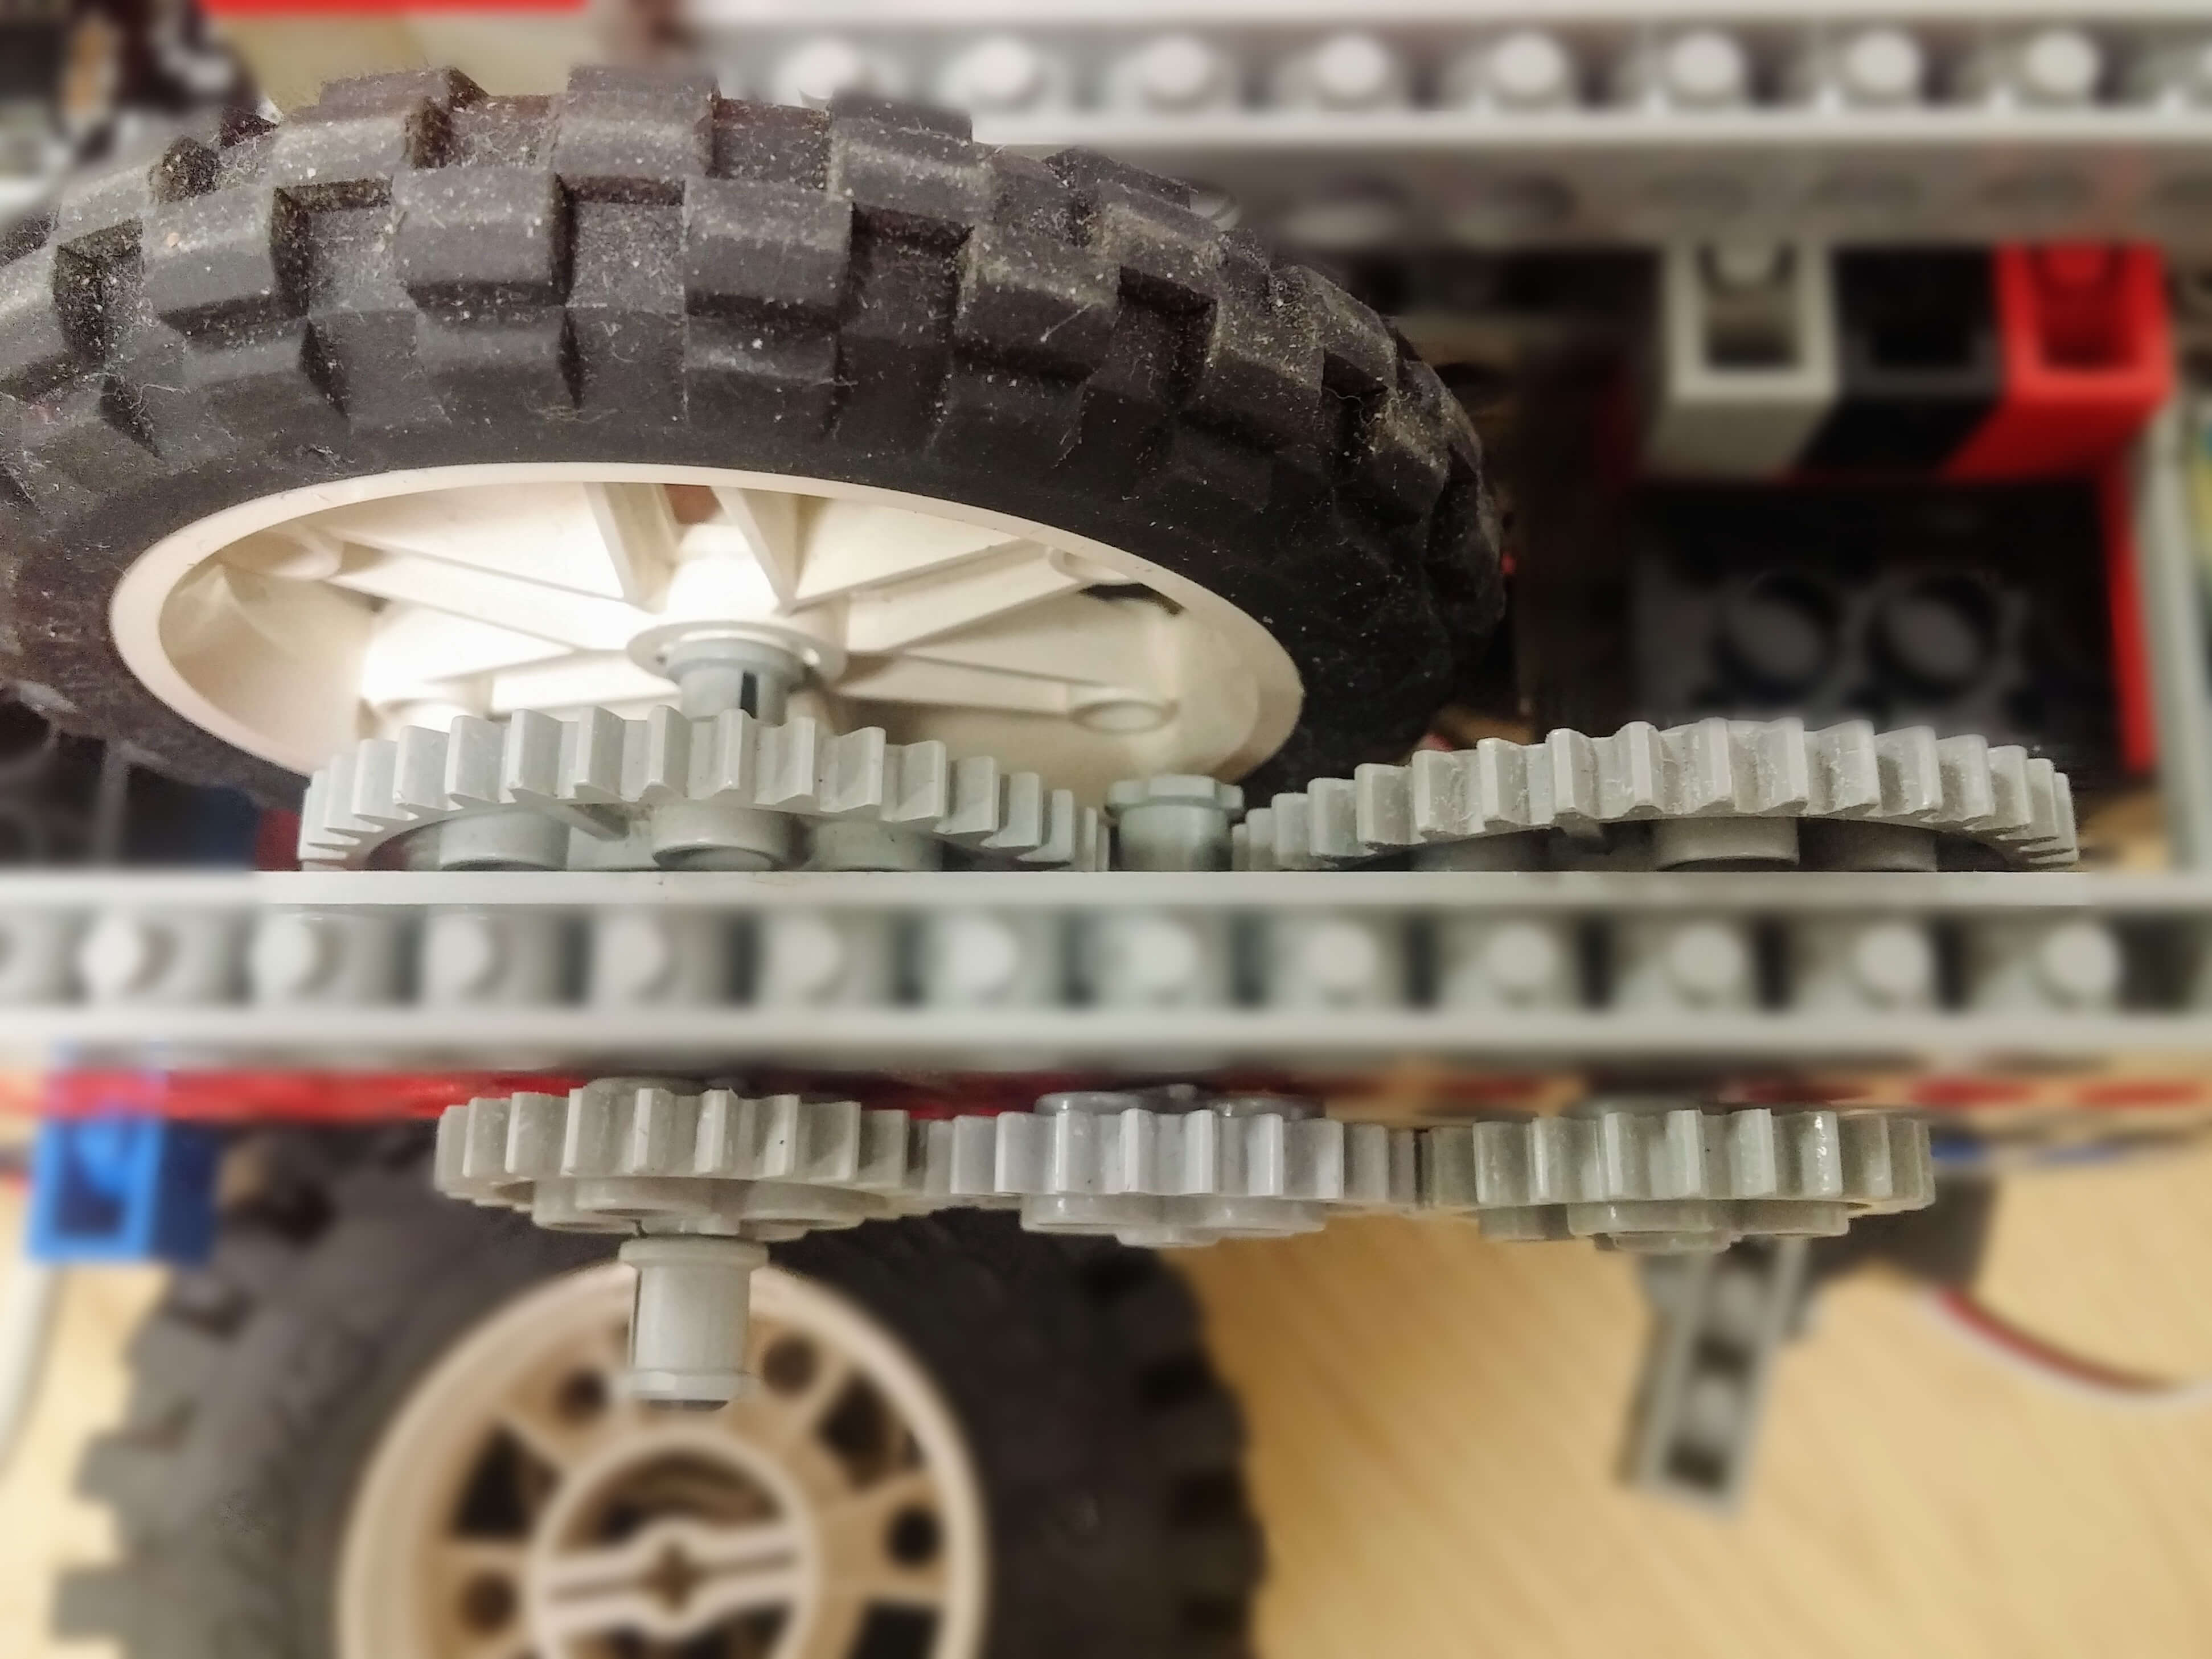
\includegraphics[width=0.7\linewidth]{res/robot-pics/gear-train-mounted.jpg}
    \caption{The assembled version of the gear train on the robot's main structure.}
    \label{fig:gear-train-mounted}
\end{figure}

% - - - - - - - - - - - - - - - - - - - - - - - - - - -

\subsection{Sensing}

This section describes the sensors used by the robot to collect inputs from its surroundings.

\subsubsection{IR and Sonar}

The robot used two IR sensors and a Sonar for its collision avoidance system and navigating on the arena.

The two IR sensors were mounted on top of the DC motors, at the front of the robot, pointing mostly forward, but each at an angle of approximately 14º outwards.

The Sonar was placed at the top of the robot, right next to the camera.

\begin{figure}[ht]
    \centering
    \begin{subfigure}{0.49\textwidth}
        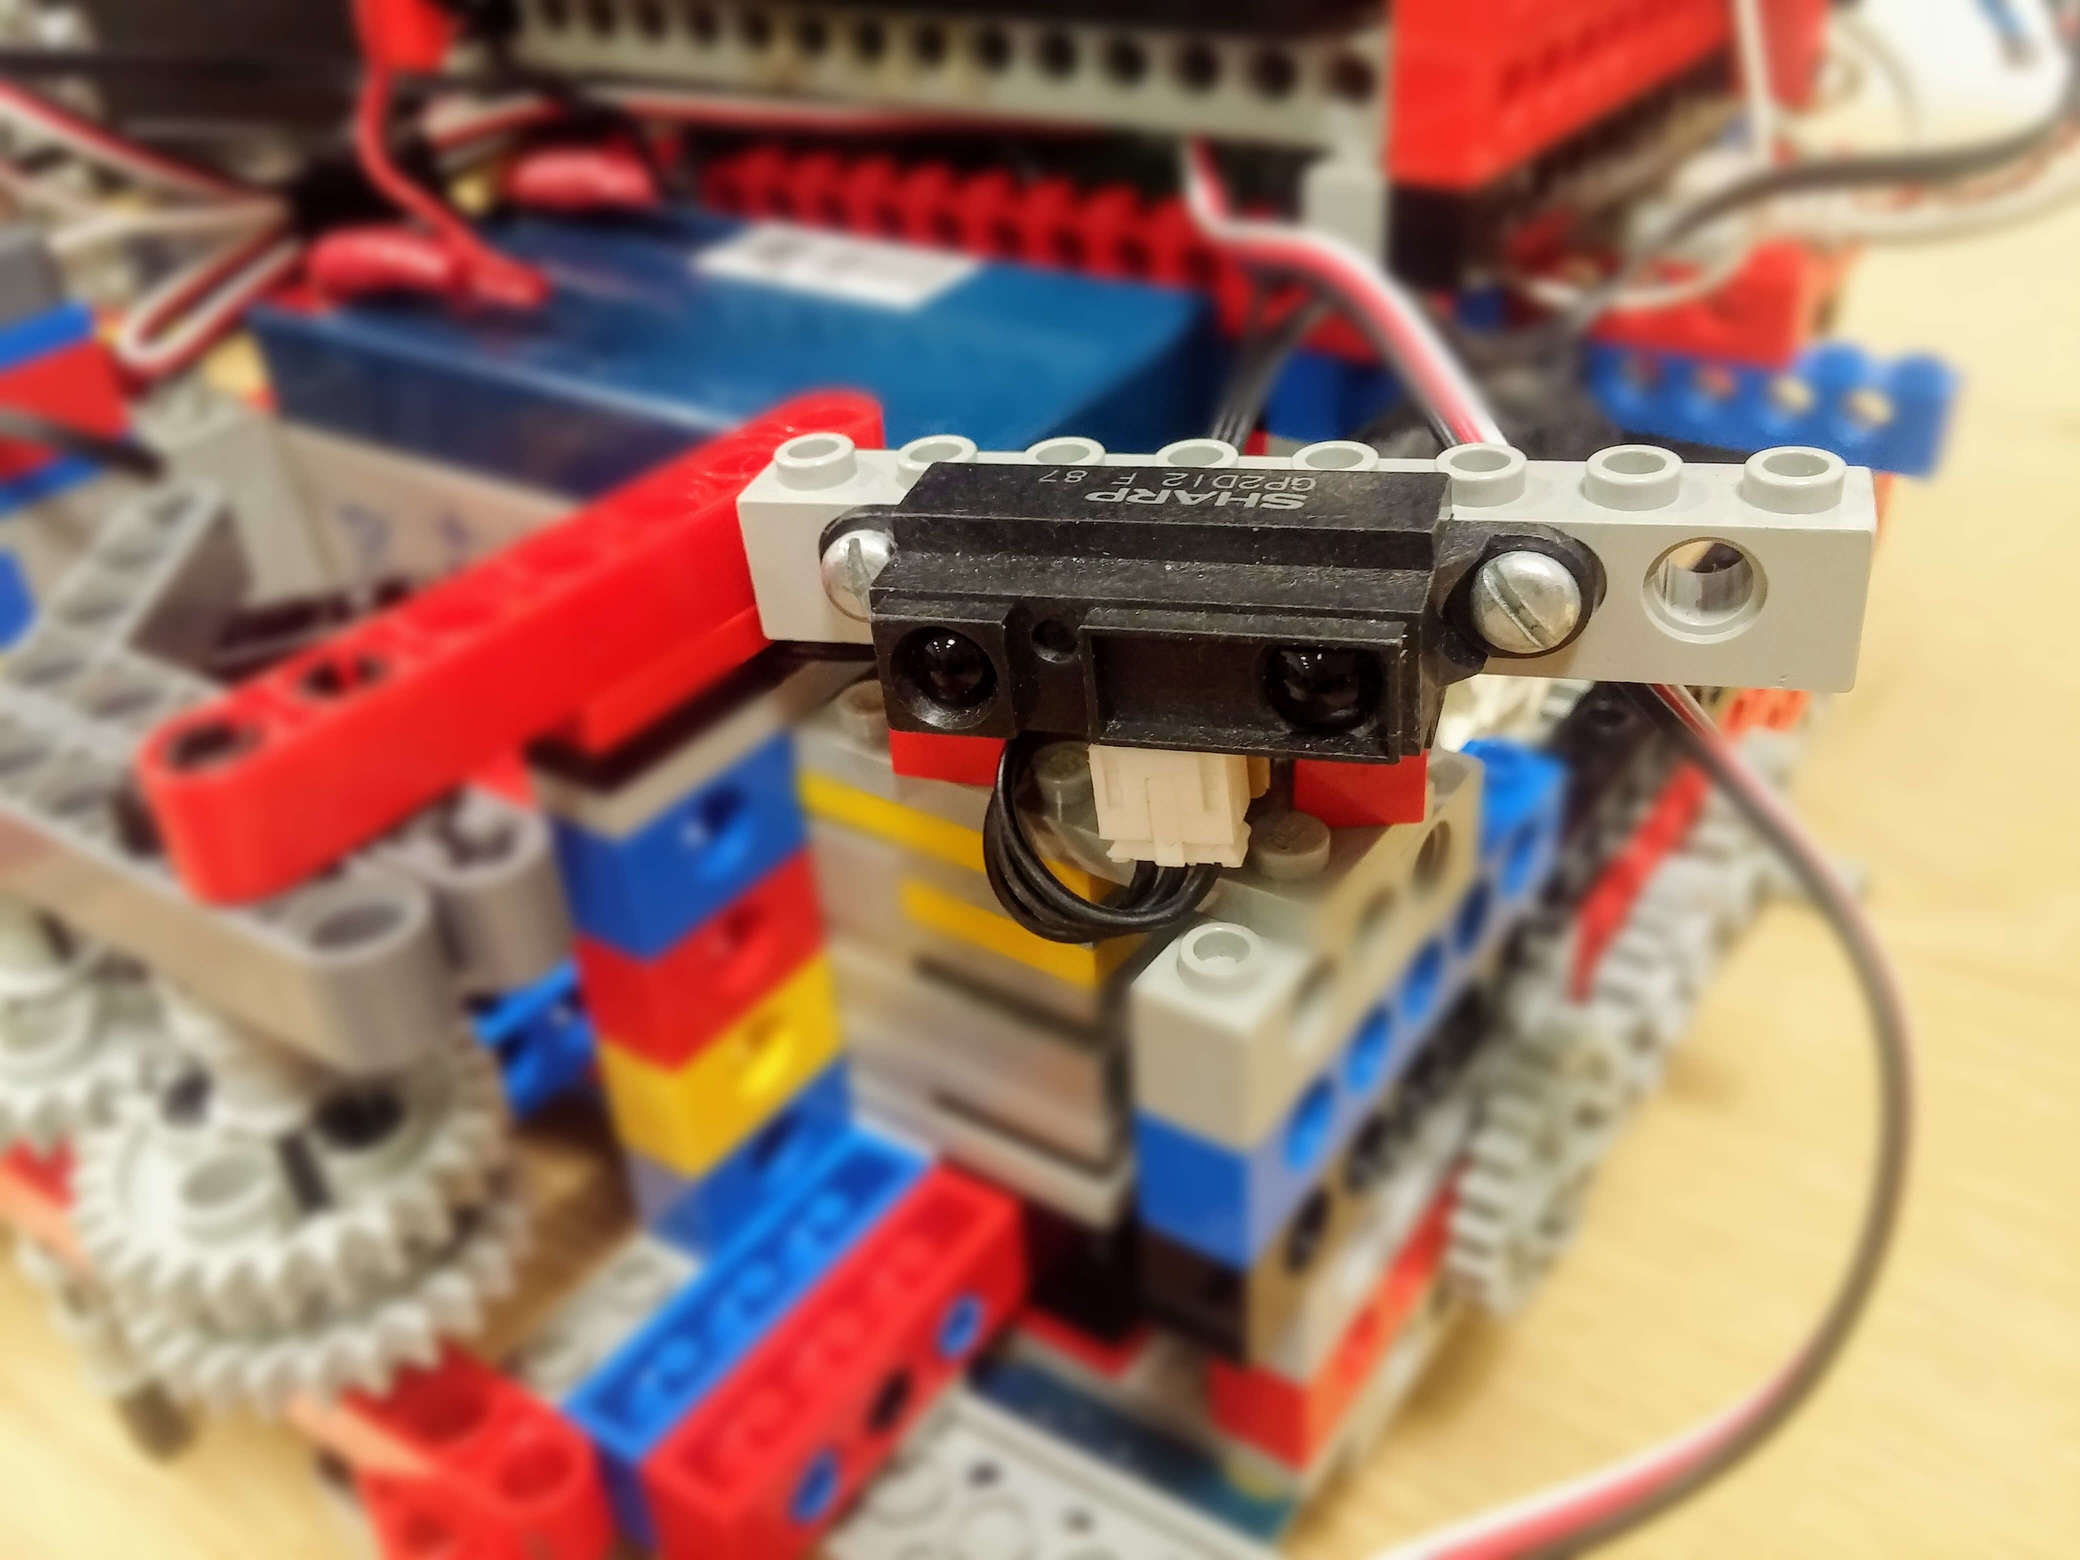
\includegraphics[width=\linewidth]{res/robot-pics/ir-sensor-placement.jpg}
        \caption{Left IR sensor}
        \label{fig:ir-sensor-placement}
    \end{subfigure}
    \begin{subfigure}{0.49\textwidth}
        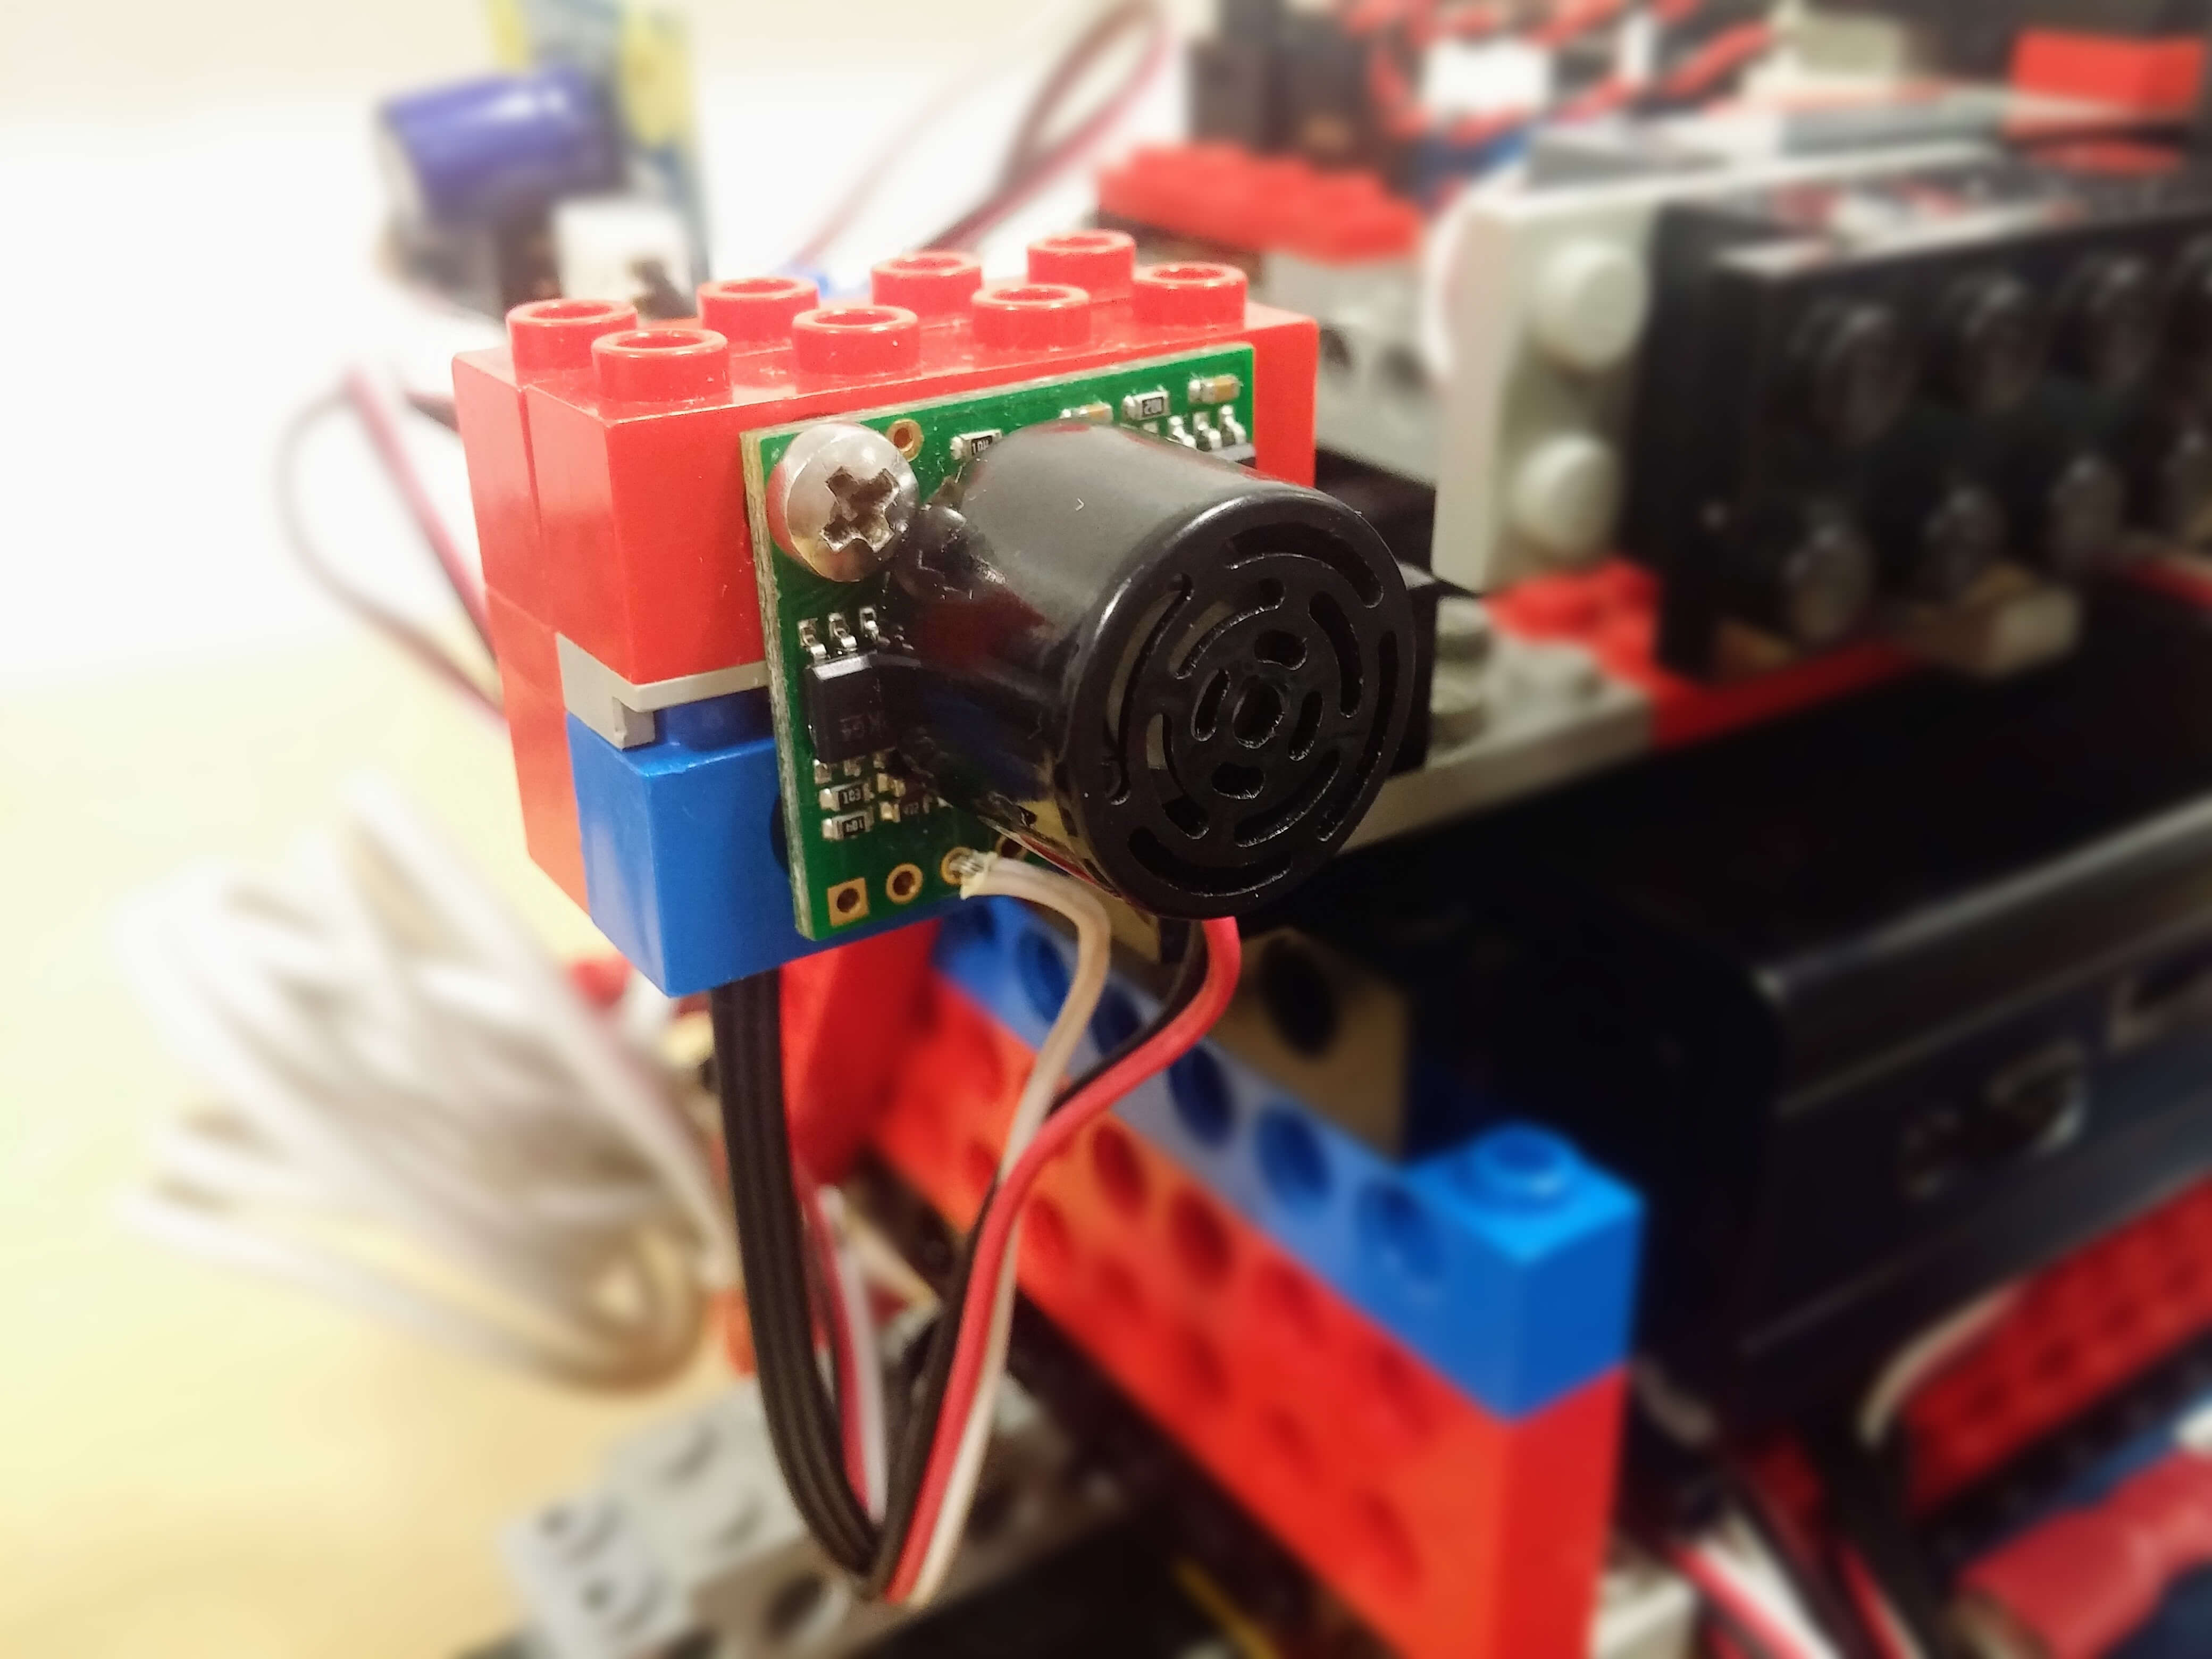
\includegraphics[width=\linewidth]{res/robot-pics/sonar-placement.jpg}
        \caption{Sonar}
        \label{fig:sonar-placement}
    \end{subfigure}
    \caption{(a) shows where the left IR sensor was placed, and at what angle. (b) shows the sonar placement, facing forwards.}
    \label{fig:ir-and-sonar}
\end{figure}

\subsubsection{Whiskers}
\label{sec:whiskers}

Up until the first major milestone the robot made use of two whisker sensors. Their purpose was to make up for the blind angle caused by the two IR sensors pointing slightly outwards. They were essential for the demonstration of the first major milestone because the robot navigated the arena randomly, and there was the possibility of it driving towards an edge of a wall without the IR sensors to get triggered. The whiskers would be triggered in such cases and would ensure the robot could back up and re-plan its route.

The whiskers have since been removed because the final robot did not have a \textit{reactive} behaviour only, it also had some \textit{planning} - and that classifies it as a \textit{hybrid} behaviour. Such planning ensured that the robot would never navigate the arena in a way that it could approach a wall edge without the IR sensors to be triggered. This turned the whisker sensors obsolete and ultimately led to their removal.

\subsubsection{Camera}

The camera attached to the top of the robot was used to scan the arena for cube resources, approaching those cubes, and identifying them.

\bigskip

\begin{figure}[ht]
    \centering
    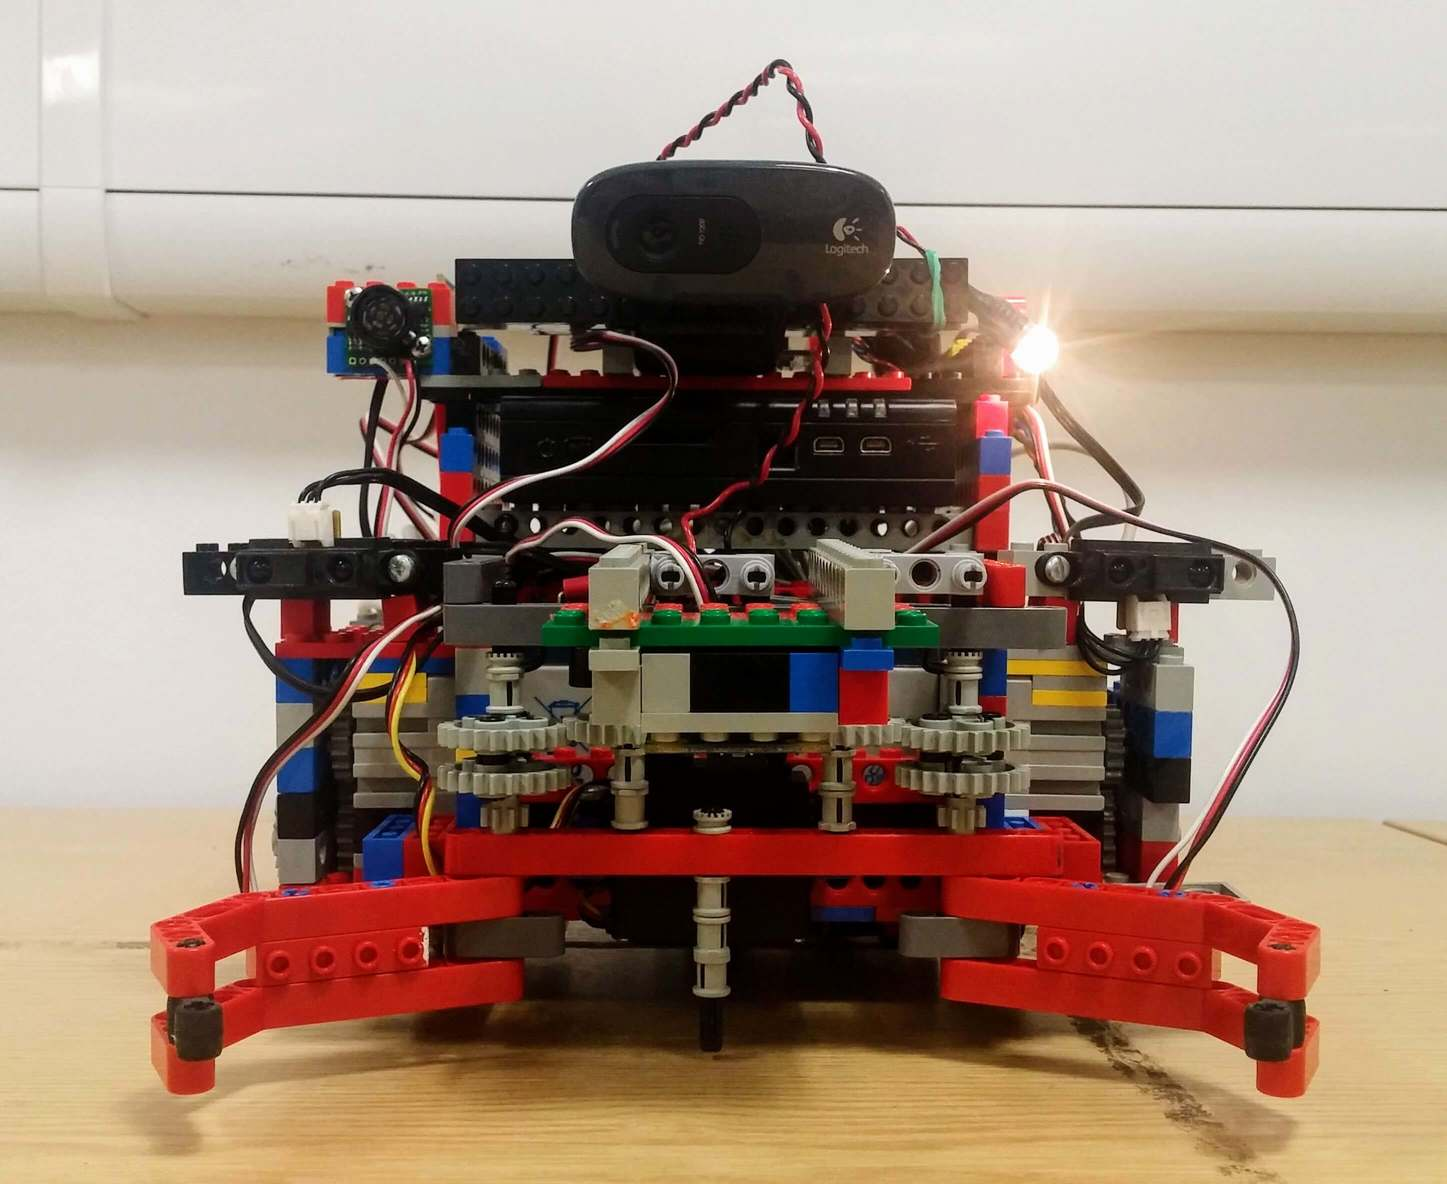
\includegraphics[width=0.7\linewidth]{res/robot-pics/view-front.jpg}
    \caption{Front view of the robot featuring the camera on the top, the Sonar to its left, and the IR sensors just below them, pointing slightly outwards.}
    \label{fig:camera}
\end{figure}

\subsubsection{Hall effect sensor}

A hall effect sensor was used for \textit{odometry} to keep track of the distance travelled by the robot.

A small pivot wheel was placed in-between the two large wheels that drive the robot, aligned with their axle. The axle on which this pivot wheel is attached transfers its rotation to a perpendicular axle, which rotates below the robot, just like a shaft, and in its turn inputs its rotation to the hall effect sensor.

\begin{figure}[ht]
    \centering
    \begin{subfigure}{0.32\textwidth}
        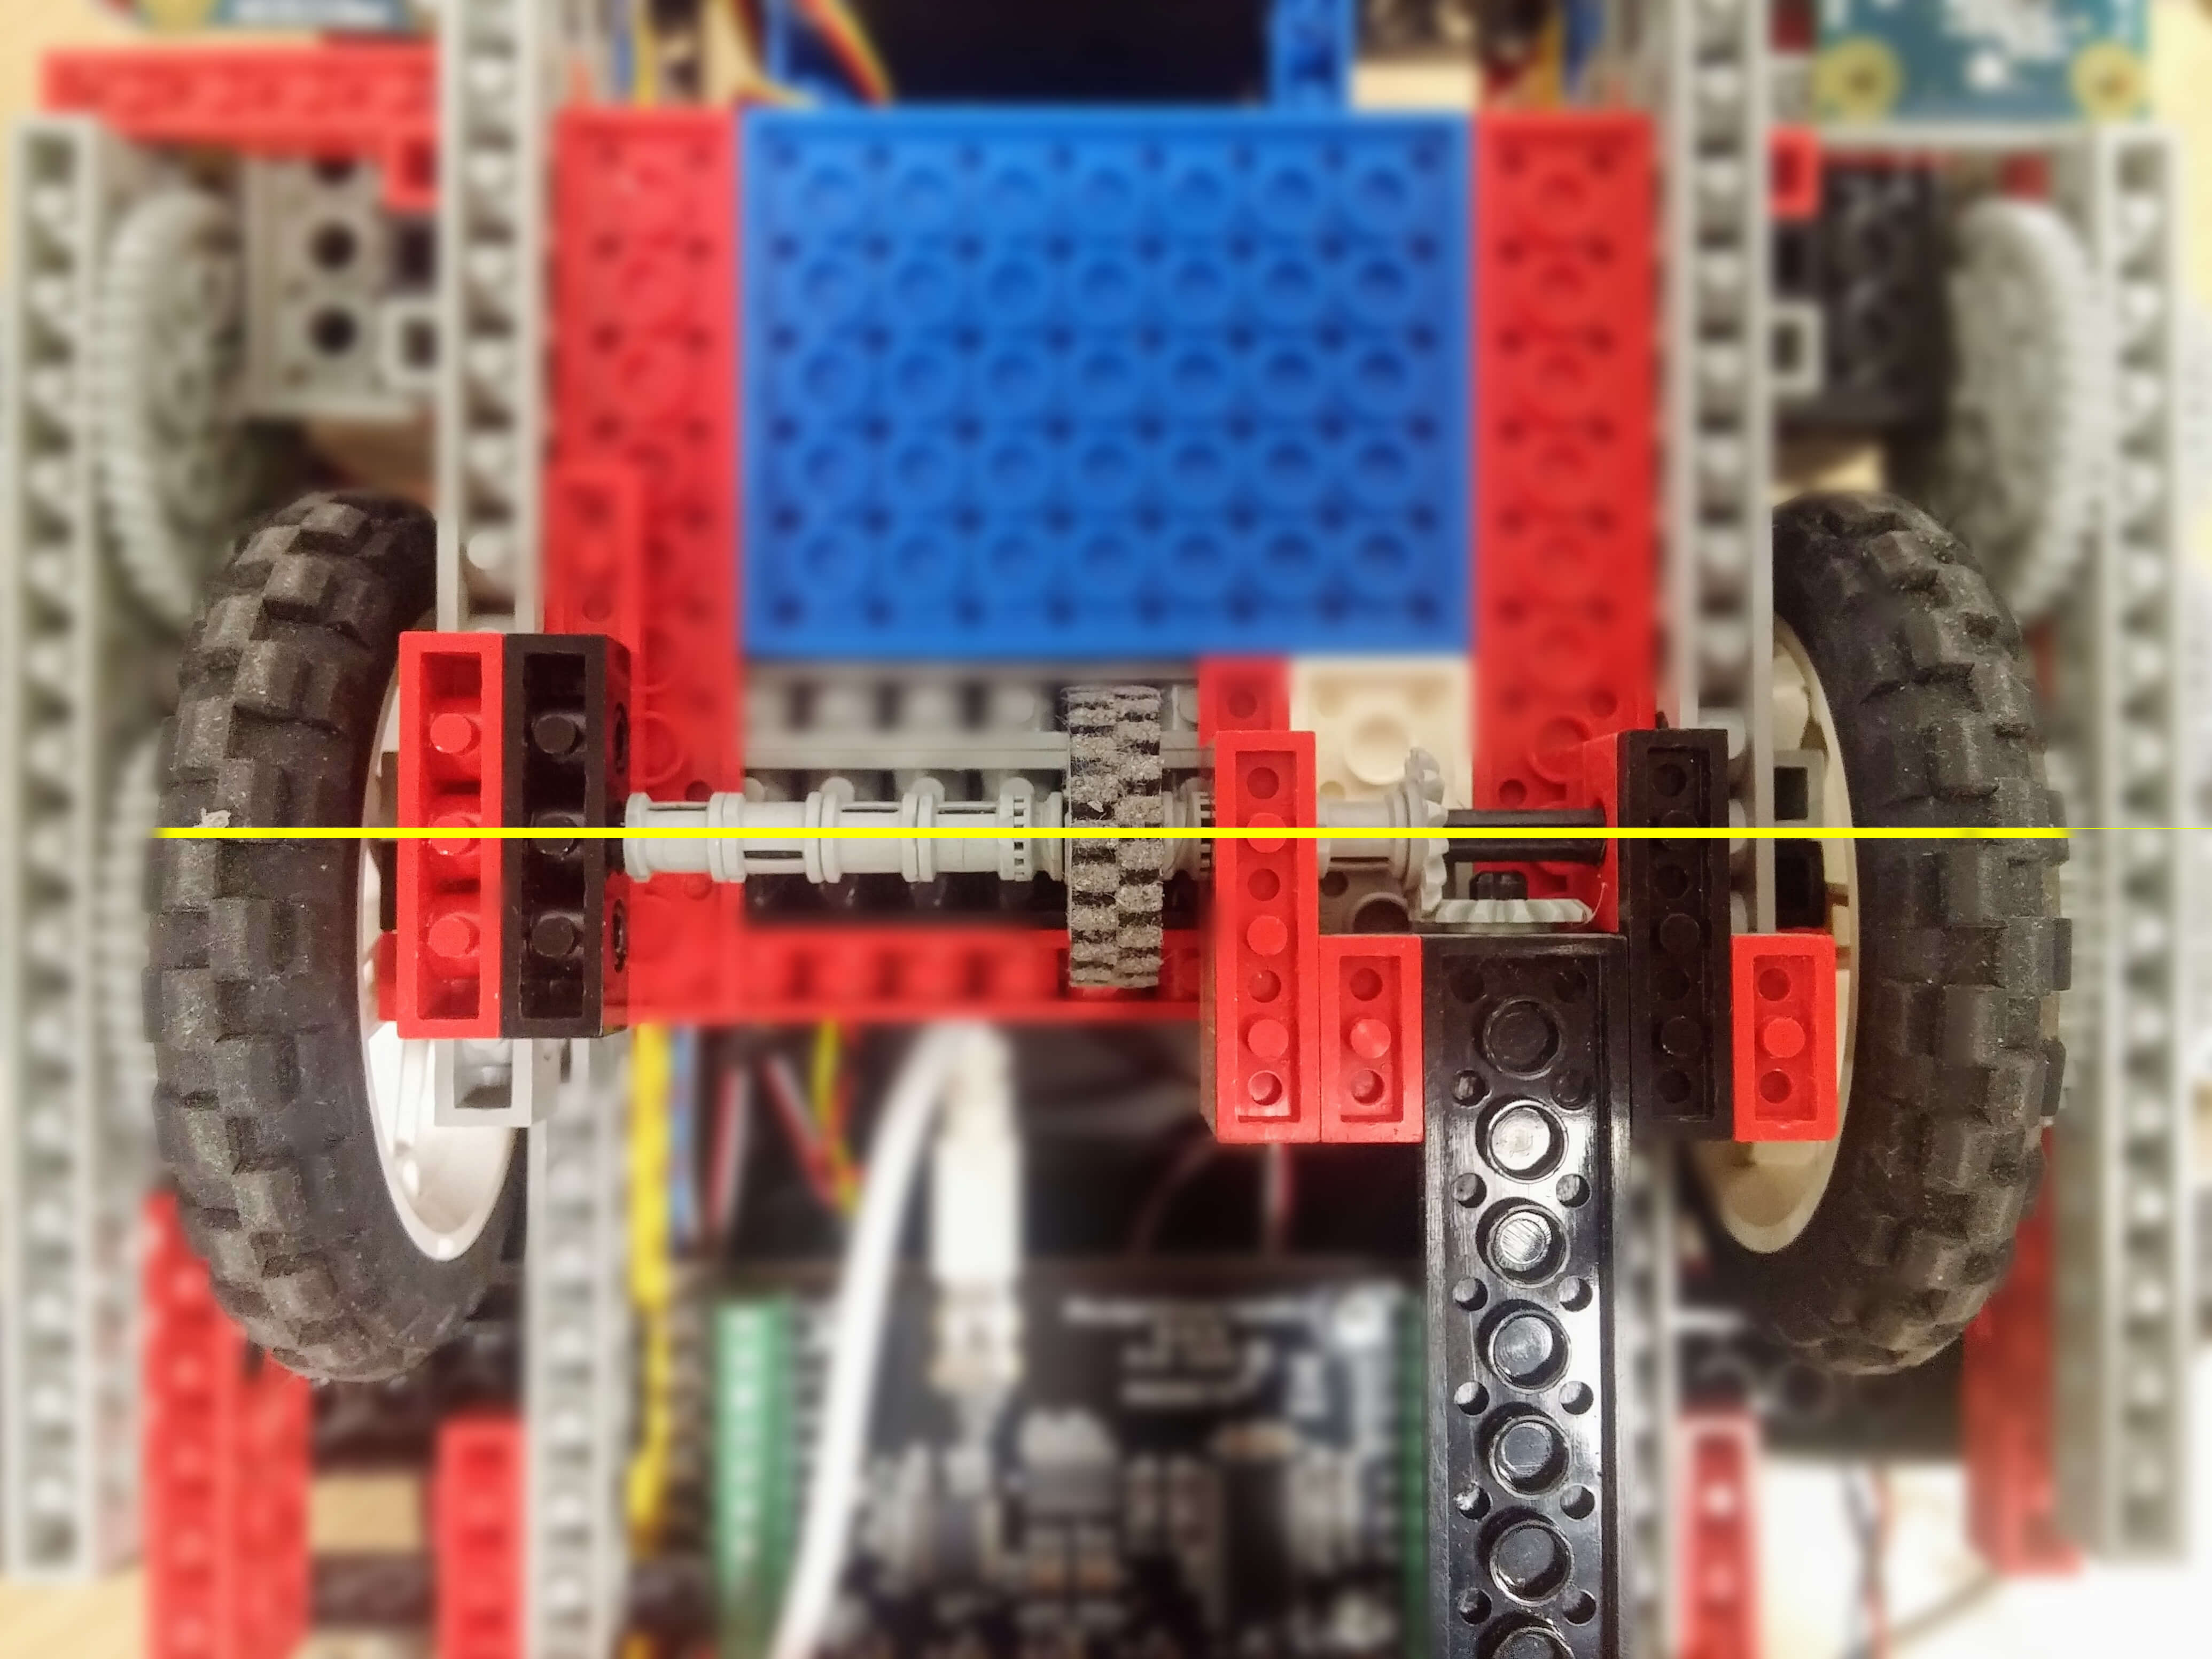
\includegraphics[width=\linewidth]{res/robot-pics/pivot-wheel-layout.jpg}
        \caption{Pivot wheel placement}
    \end{subfigure}
    \begin{subfigure}{0.32\textwidth}
        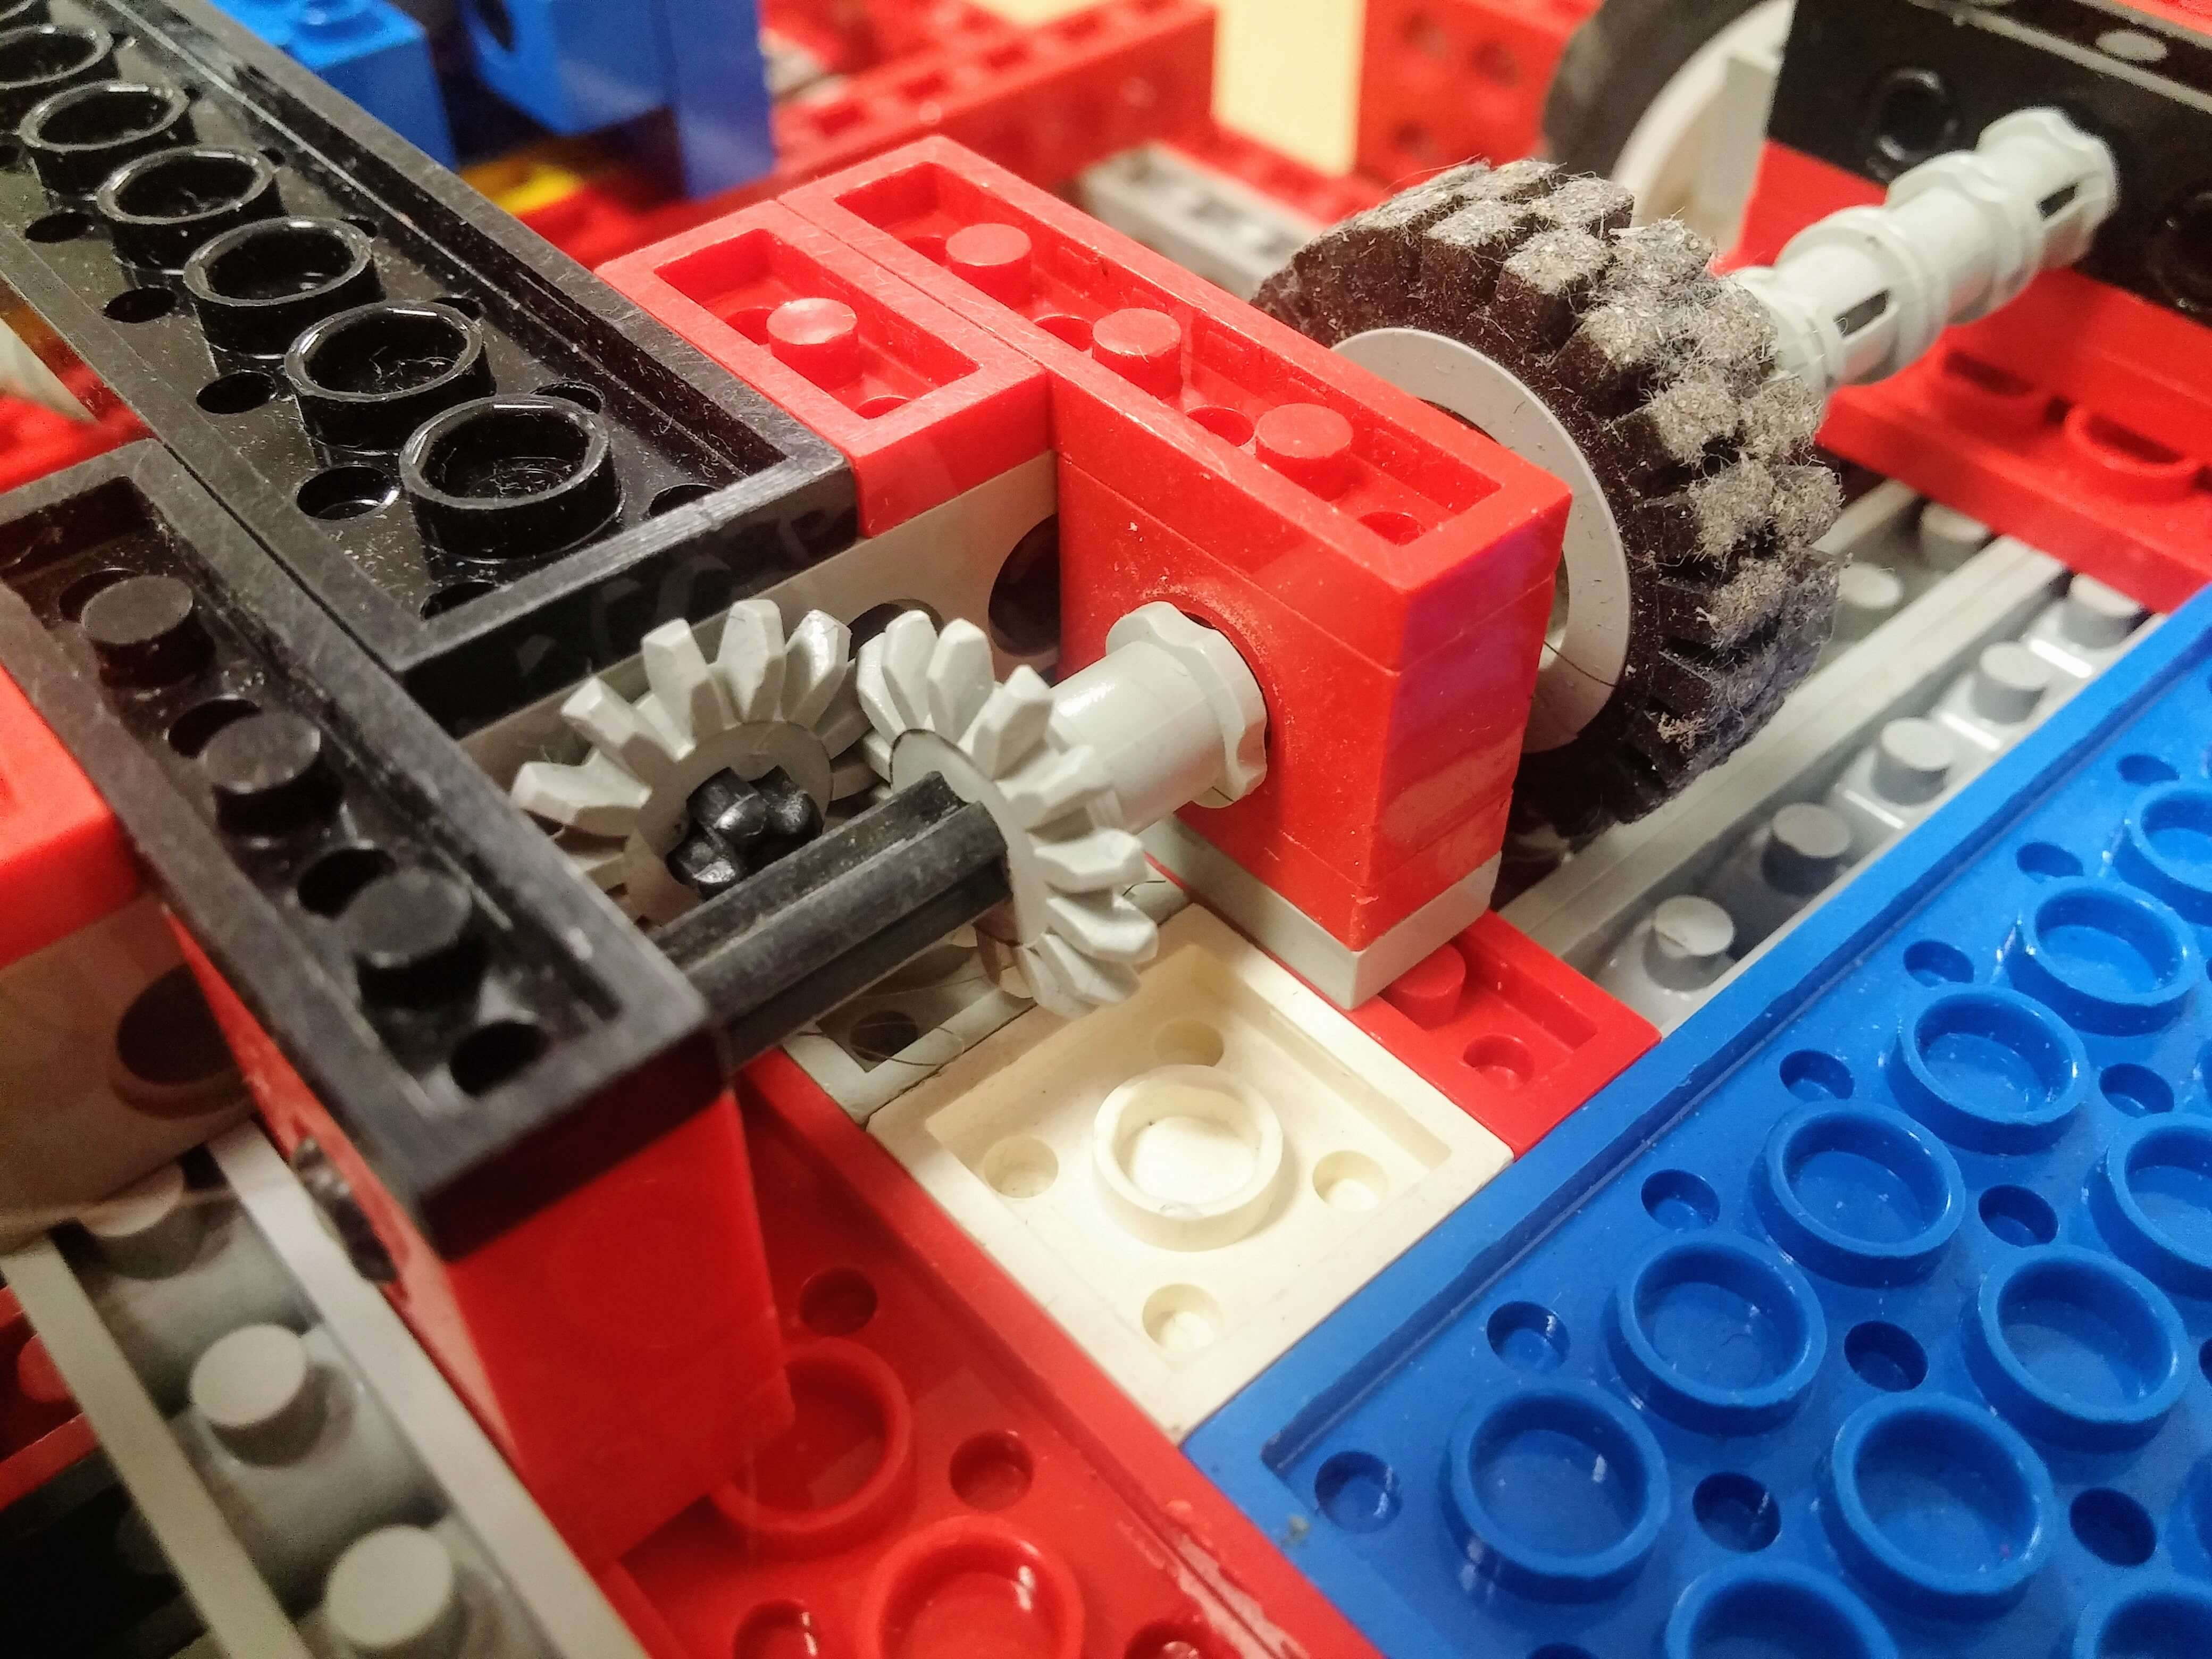
\includegraphics[width=\linewidth]{res/robot-pics/pivot-wheel-axel-transfer.jpg}
        \caption{Axle transfer}
    \end{subfigure}
    \begin{subfigure}{0.32\textwidth}
        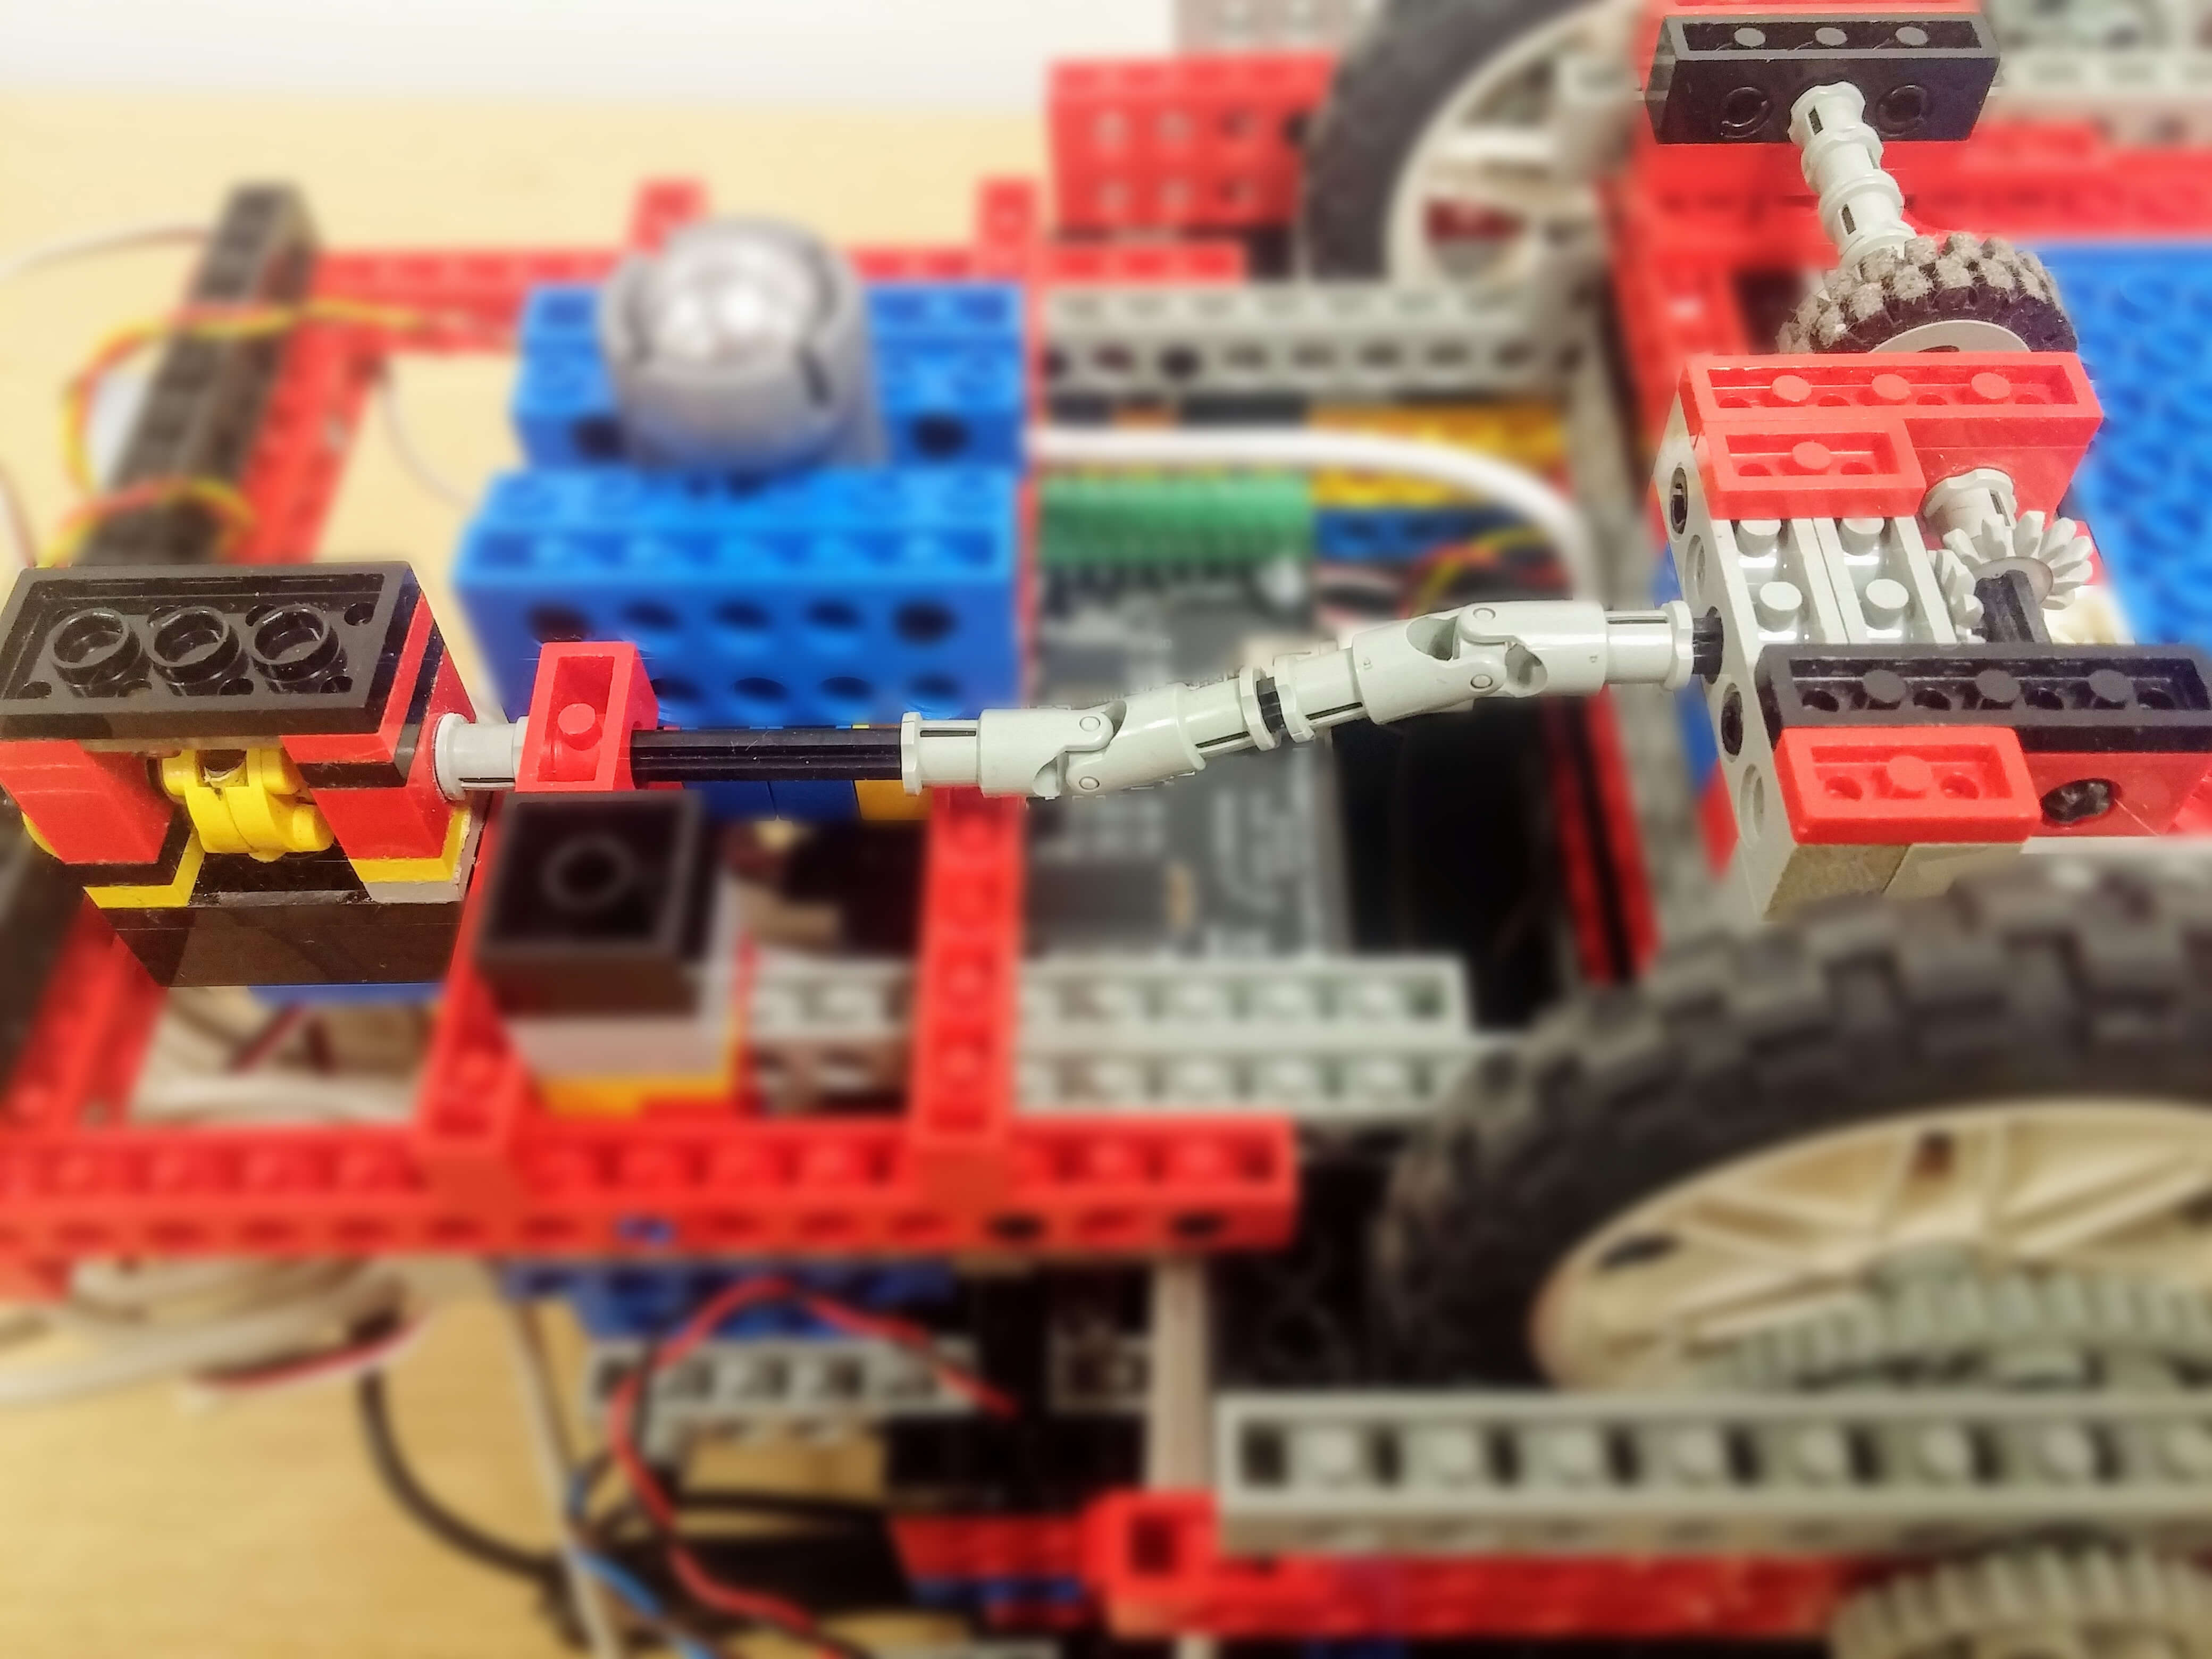
\includegraphics[width=\linewidth]{res/robot-pics/pivot-wheel-sensor.jpg}
        \caption{The whole mechanism}
    \end{subfigure}
    \caption{(a) shows the placement and alignment of the pivot wheel. (b) shows gearing to transfer the rotation from the pivot wheel axle to the shaft. (c) shows the entire mechanism, from the pivot wheel to the hall effect sensor.}
    \label{fig:pivot-wheel-system}
\end{figure}

% - - - - - - - - - - - - - - - - - - - - - - - - - - -

\subsection{Logical architecture}

All the source code of the robot was programmed in \textbf{Python 2.7}, and has been made publicly accessible on its entirety at \url{https://github.com/ferrolho/uoe-rss}.

\begin{figure}[ht]
    \centering
    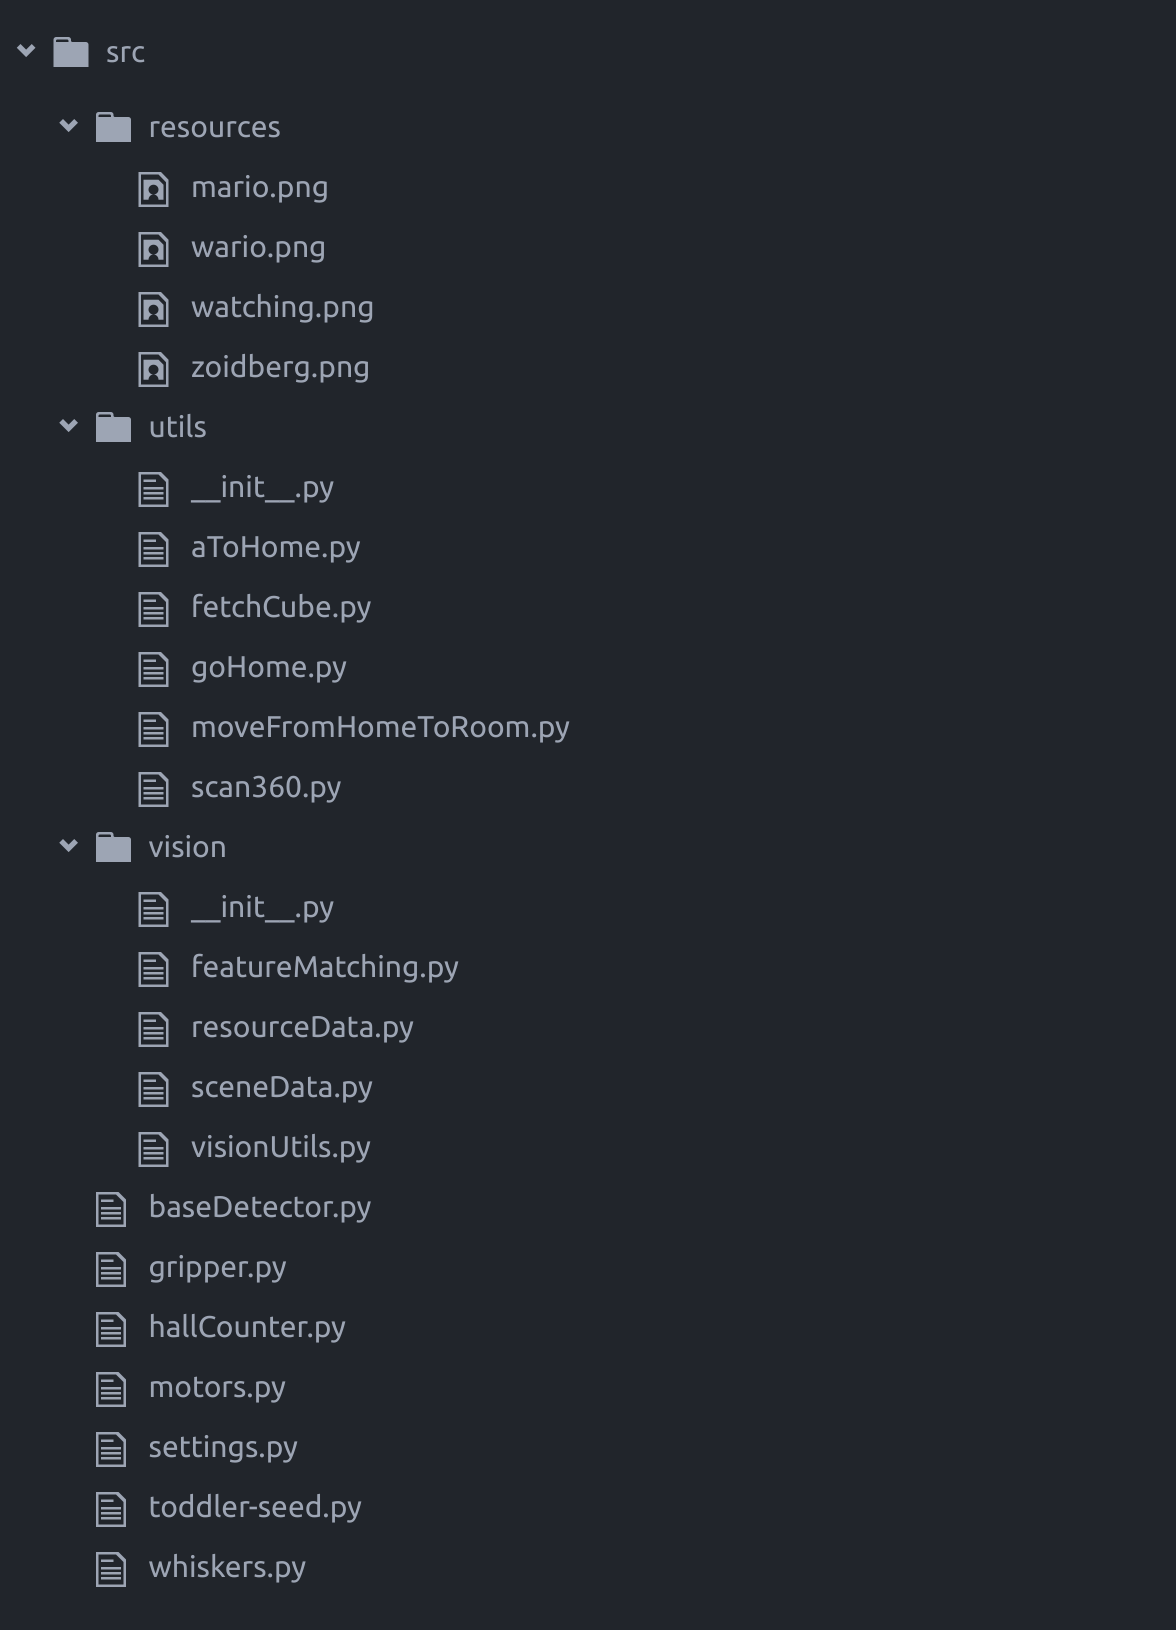
\includegraphics[width=0.45\linewidth]{res/source-architecture.png}
    \caption{The source code file structure and modules.}
    \label{fig:source-architecture}
\end{figure}

\clearpage

\subsubsection{The \texttt{src/} root folder}

The \texttt{src/} folder is the root of the project. It contains two modules: \textbf{utils} and \textbf{vision}, the \textbf{resources} folder, and other source code files.

The \texttt{resources/} folder contains all the four different textures that the robot could find while navigating through the arena.

\texttt{settings.py} is where the main configurations for the robot are, including the assignment of each resource to one of the bases of the arena.

\texttt{baseDetector.py} is the the class that abstracts and interfaces the two light sensors responsible to detect the two black rectangular bases of the arena.

\texttt{gripper.py} is the class that abstracts and interfaces the gripper. Convenient methods to close and open the gripper exist, as well as methods to check if there is a cube on the gripper.

\texttt{hallCounter.py} is the class that processes the measurements of the hall effect sensor. It keeps track of the total distance travelled by the robot. Also contains a handy method to set a timer which goes off after the robot as travelled the distance set by the \texttt{setTimer()} function.

\texttt{motors.py} is the class that interfaces the motors. Multiple simple behaviors have been abstracted to make the development easy. For example, to make the robot move forward, one needs only to call \texttt{self.moveForward()}.

\texttt{whiskers.py} is the class that abstracts the whiskers.

\texttt{toddler-seed.py} contains the \texttt{Toddler} class, and is the main program, and the starting point of the robot control flow. The class implements a \textit{Finite State Machine}, which can be summed up in the following keypoints:

\medskip

\begin{enumerate}
    \centering
    \item Scan 360 for a room
    \item Move into that room
    \item Search for and fetch the cube
    \item Deliver cube to the respective base
    \item Return home
\end{enumerate}

% - - - - - - - - - - - - - - - - - - - - - - - - - - -

\subsubsection{The \texttt{utils/} module}

The \texttt{utils/} module contains all the high-level source code for the fundamental procedures to solve the task.

\texttt{scan360.py} is a high-level procedure which implements a simpler state machine to solve the first problem of the task, i.e., when the robot was placed on the center of the arena, facing a random direction, this procedure was the one responsible to turn the robot until it was facing the room entrance of interest.

\texttt{moveFromHomeToRoom.py} this procedure is the one responsible to plan the robot route from home (the center of the arena) to the room of interest. It assumes that the 360 scan had been ran previously, and as such, that the robot was already facing the room it wanted to move into.

\texttt{fetchCube.py} is the routine responsible for scanning the room for a cube resource, and when it spots a cube, approaching it and locking it on the robot's gripper.

\texttt{goHome.py} is the high-level abstraction to return home assuming the robot had just delivered a cube to the base in room B.

\texttt{aToHome.py} is pretty much the same as \texttt{goHome.py}, the difference is on the planning routine to go home for cases when it is assumed the robot just delivered a cube to the base on room A.

% - - - - - - - - - - - - - - - - - - - - - - - - - - -

\subsubsection{The \texttt{vision/} module}

The \texttt{vision/} module contains all the source code required to process and extract important information from the images taken by the robot's camera.

\texttt{sceneData.py} and \texttt{resourceData.py} are two simple and very similar classes that represent the information stored on a frame, i.e., a frame keypoints and descriptors, which are required to run the SIFT algorithm.

\texttt{featureMatching.py} is the source file which contains the function to run the SIFT algorithm between two images.

\texttt{visionUtils.py} is the most important class of the module, and creates a level of abstraction for sub-tasks like scanning for cartoons on an image, and looking for a cube in the distance.

\newpage
